\documentclass[12pt,a4paper]{article}

% Header and footer stuff
\usepackage[left=3.5cm,right=2cm,top=3.5cm,bottom=2cm,includefoot]{geometry}
\usepackage{fancyhdr}
\pagestyle{fancy}
\fancyhead{}
\fancyfoot{}
\fancyfoot[R]{\thepage}
\renewcommand{\headrulewidth}{0pt}

\usepackage{mathptmx}
\usepackage{graphicx}
\usepackage{float}
\usepackage[hidelinks]{hyperref}%Allows for navigation to the topic by clicking on Table of 		                         contents
\usepackage{amsmath}
\usepackage{relsize}

\linespread{1.2}

%Here Begins the document
\begin{document}


%For Acknowledgements Portion
\pagenumbering{roman}
\section*{ACKNOWLEDGEMENT}
\addcontentsline{toc}{section}{\numberline{}ACKNOWLEDGEMENT}
We would like to express our deepest gratitude to Department of Computer Engineering for providing us this huge opportunity to utilize and explore our skills through this project.\\ \\
We extend our sincere gratitude to Asso. Prof. Manoj kr. Halwai providing us the necessary guidelines for the project. \\ \\
We extend our vote of thanks to everyone who have provided their cooperation, guidance and constructive criticism in this project.

\cleardoublepage{}

\section*{ABSTRACT}
\addcontentsline{toc}{section}{\numberline{}ABSTRACT}
For so long, many institutions, especially academic ones, have been throttled to posting notice messages physically up at a notice board. A Notice Board is a place where people can leave public messages, for example, to advertise things, announce events, or provide information. Besides the low audience that this method has often seen, the notices suffer from staleness and non-portability. In an attempt to solve these problems, several notice broadcasting techniques around the globe have been tested. These may include electronic screens, which may solve all but the latter problem: portability.\\ \\
Hence, we have proposed a Online Notice Board web application that will help in solving problem of information flow among different stakeholders. Online Notice board is a web application which is engaged in providing up- to-date articles and notices and other information’s for all the users or student associated with the particular campus or department. The project aims at, how the online notice board can improve the efficiency of the student when it comes to gaining the information from the college. Online notice board is one of the applications to improve the usage of notice board of the college by making it available online.


\cleardoublepage{}

%Table of contents
\tableofcontents
\thispagestyle{empty}
\cleardoublepage{}

%List of figures
\listoffigures
\addcontentsline{toc}{section}{\numberline{}LIST OF FIGURES}
\cleardoublepage{}

%Body
\newpage
\pagenumbering{arabic}
\setcounter{page}{1}
\section{INTRODUCTION}
The introduction of the internet in the 1950’s has offered the world a new idea to the continuously developing IT world. Several uses of the internet
have since been adopted with applications in commerce, communications and media \cite{internet} \cite{internet2}.\\ \\
The Online Notice Board System is intended for colleges and institutions where information sharing on regular basis plays vital role in the performance. The proposed system will act as an online notice board which will make use of the modern communication methodologies and techniques for information flow. The system is planned to consist of various useful features for the said purpose. The proposed system aims to create a platform for issuing notice, sharing information between the members of the institution. Different users shall have different level of access to the content. In the context of a college, there shall be three users of
the software – administrator, student and guest. The administrator shall be
able to issue notice and view students’ activities on the software. The student shall be able to view the notices intended for them. A guest will simply be able to view public notices.\\

	\subsection{PROBLEM STATEMENT}
	In today’s world, everything is digitized and paper is being used less and less every day. How often has it happened that we miss some important notice because we have to go to a wall and read the notice there? There are dedicated file hosting sites and clouds used by some institutions, but there is a definite need for a dedicated noticeboard system. The proposed system is such a system. Some of the major problems are highlighted below:
	\begin{itemize}
	    \item difficulty in information flow to each individual
	    \item the concerned party may not be physically available near the notice board to consume the information
	    \item historical notices removed\\
	\end{itemize}
	
	\subsection{NEED}
	Almost all leading institutions, excepting a few, currently lack an electronic noticeboard system. Though some have taken the aid of third-party websites like Facebook® to interact, it comes at the cost of mixing one’s social life with professional. Keeping this in mind, educational institutes will find this software extremely useful.\\
	The “Online Notice Board System” is a web- based software, with supplementary application software, that aims to aid the institutes by providing such digital noticeboard.\\
	
	\subsection{SOLUTION TO THE PROBLEM}
	Instead of relying on admin or teachers for updating the notice on notice board every time, it would be better if we make proper use of information technology for achieving our goal. We can easily deploy a system in educational institutions like colleges that can handle the problem of information and notification flow across that organization. The proposed system can solve our problems in following ways:
	\begin{itemize}
	    \item the system should enable easy and fast access to all records
	    \item the system should provide better data management facilities
	    \item reduction of paper notices and notice boards
	    \item easy and fast updates of records
	    \item there should be some security measures to prevent unauthorized manipulation of notices\\
	\end{itemize}
	
	\subsection{OBJECTIVES}
	The primary aim of the Online Noticeboard Software project is to create a fully functional digital noticeboard system which will efficiently handle all assigned tasks. It may be able to, in due course, heavily minimize, if not eradicate, the conventional, physical noticeboards. With the help of the supplementary applications, users will be able to receive real-time notifications of any and all notices posted by another user with privileges as such.
	\begin{itemize}
		\item to develop supplementary apps for the said noticeboard
		\item to create a user-friendly interface
		\item to develop and manage a proper database system to ensure data safety and proper management
		\item to allocate various levels of users and have proper authentication
		\item to prepare proper and detailed system documentation\\
	\end{itemize}
	
	\subsection{SCOPE}
	The system covers issuing public as well private notifications to all the users. Public notifications are intended for all the users while the private notifications are targeted to a particular individual. The system performs validation on input data and maintains consistency across different files as well to some extent.

\newpage
\section{FEASIBILITY ANALYSIS}
This section deals with the technical, schedule, economic, operational, legal, religious-cultural and socio-political feasibility that can arise during development of this project.

    \subsection{TECHNICAL FEASIBILITY}
    The software is to be developed using HTML, PHP, CSS and MySQL, which are all readily available. Also, the team members have sufficient programming and related knowledge which will enable us to learn and adapt to these specific languages and platforms easily. Thus we can see that the project is technically feasible.
    
    \subsection{SCHEDULE FEASIBILITY}
    The development process is planned to reach designing phase till the end of the semester, which gives us a windows of roughly six months. Although this may be a tight fit for a perfect, final system, as the Incremental Model is being followed in the SDLC, this is enough time to develop a working first version of the software.
    
    \subsection{ECONOMIC FEASIBILITY}
    The program uses programming languages whose IDE are freeware. We mostly made use of Sublime text editor which is publicly available for free of cost. Further costs for this project are the costs of online domain, space and database and registering and uploading the apps in the respective market, which is expected to be covered by the college. The remaining cost is that of training the developer team in the particular language and/or platform, which is minimal. So the project is economically feasible.
    
    \subsection{OPERATIONAL FEASIBILITY}
    The software requires very little specific environment to run. Only the apps require their environment to run, i.e. Windows 8™. As a staggering majority of the PCs in the world are based on Windows™ OS, this cannot really be considered a need. The software will be extremely user-friendly, removing the need for specifically trained employees. Similarly, the cost of buying the rights and the maintenance cost will not be very high for the client. So the software is feasible for operation.
    
    \subsection{LEGAL FEASIBILITY}
    The developers will obviously use no illegal means or methodologies in the development process of the system. The software will be built and operated abiding by the Cyber and other applicable laws prevailing in the country enforced by the Government of Nepal. The user will be held responsible for only the data they enter to the system. In case of international users, they will be subjected to the applicable laws in that country. So the software has no legal barrages.
    
    \subsection{RELIGIOUS-CULTURAL FEASIBILITY}
    This system will never ask the user of their religion or cultural origin and ergo will not act in any way whatsoever that may hurt the sentiments of any cultural or religious group. The product development or operation will never undergo any process that might be unacceptable to a specific religion or culture. The software itself will be generic and impartial. So no religious or cultural issues should disrupt the system.
    
    \subsection{SOCIO-POLITICAL FEASIBILITY}
    This software, being a simple notice board system, will by no means cause any alarms or questions in the society nor will it challenge any existing social conventions. Further, the software will not contradict or interfere in any way with the political happenings. The software will not be used as a means of campaign or promotion or a specific political or social organization. So the software is socially and politically feasible.

\newpage
\section{RISK ANALYSIS}
This section deals with all the risks involved with the implementation of the proposed system.

    \subsection{PERFORMANCE RISKS}
    The software performance may be hampered due to various factors like unresponsive UI and failure to execute given command(s). One of the factors for these can be a large-sized front end, which can be corrected by making a lightweight UI. The other reason for this can be poor internet connection or client-side faults, and are outside the control of the developers. The use of a middleware also hampers the performance so it is advisable to design the system such that front and back end can communicate directly.
    
    \subsection{SAFETY RISKS}
    Another risk with the system is the safety of the user data. The user data may be lost or corrupted if not for proper management and storage. This can be negotiated by using reliable databases in the back end.
    
    \subsection{SECURITY RISKS}
    A major risk in the system is the security of user data as well as their personal information. Firstly, the user authentication will have to be very stringent. The communication between UI and database should be secure. The database itself should be secure and measures like hashing and password protection should be used. The user’s private information should never be accessible without the express permission of the user in question.

\newpage
\section{METHODOLOGY}
Online Notice Board System is a mini project developed with a view to meet the basic requirement of handling information flow to all the concerned stakeholders within an organization.\\

    \subsection{REQUIREMENT ANALYSIS}
    The project is developed with a view to cover notice information flow of an organization. Requirement gathering in this project was mainly done through study at different educational institution. We collected information about the basic flow required for the system. These tactics helped a lot in providing a clear view of the Online Notice Board system. After gathering and analyzing the client requirement, it was represented by use case and then the system design and development started.\\
    
    \subsection{TOOLS AND TECHNIQUES USED}
    Following development tools and techniques were used for the development of this system:
    \begin{itemize}
        \item HTML
        \item CSS
        \item PHP
        \item MySQL
        \item XAMPP Server
        \item \LaTeX. for documentation
        \item Online tools for system flow diagrams\\
    \end{itemize}
    
    \subsection{SYSTEM DESCRIPTION}
    The proposed system is Online Notice Board system which is expected to fulfill basic requirements of a notice board.\\
    The system initially starts with a login process. The user of system has to enter a username and password. The entered username and password are matched with that stored in database. If the credentials are correct, then the user is allowed to login to the system and he/she can perform further operations. If the credentials are incorrect or if username or password do not match, then the user can not proceed ahead into the system.
	\begin{figure}[H]
		\centering
		\includegraphics[height=3in]{figures/login.png}
		\caption{Login Process}
	\end{figure}
	\noindent There are three levels of users basically:
	\begin{enumerate}
	    \item The guest do not need to login and can view the public notices.
	    \item The admin can login with admin credentials and they can manage users and manage notifications for each users.
	    \item The user need to register themselves into the system and afterwards, they can login into the system and manage their user accounts and notifications incidents.
	\end{enumerate}
	
    \cleardoublepage{}
	\subsection{SYSTEM FLOW DIAGRAMS}
	The system design for this problem is based on scientific approach. The following diagrams depicts the organization of our system.
	
	    \subsubsection{Use Case Diagram}
	    \begin{figure}[H]
    		\centering
    		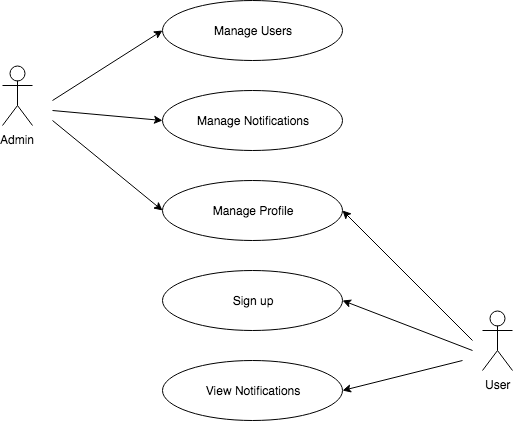
\includegraphics[height=2.5in]{figures/use_case_diagram.png}
    		\caption{Use Case Diagram}
    	\end{figure}
    	
    	\subsubsection{Class Diagram}
    	\begin{figure}[H]
    		\centering
    		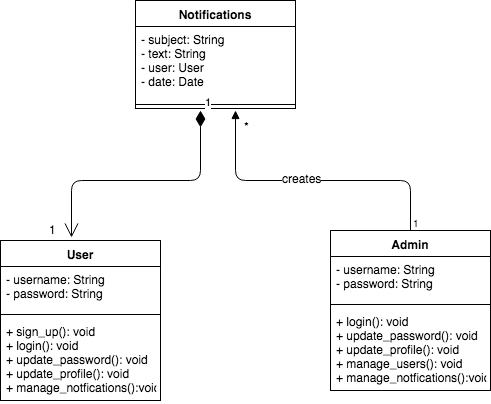
\includegraphics[width=\textwidth,height=6in]{figures/class_diagram.png}
    		\caption{Class Diagram}
    	\end{figure}
	    
	    \subsubsection{Activity Diagram}
	    \begin{figure}[H]
    		\centering
    		\includegraphics[height=6in]{figures/activity.png}
    		\caption{Activity Diagram}
    	\end{figure}
    	
    	\subsubsection{Context Level Diagram}
    	\begin{figure}[H]
    		\centering
    		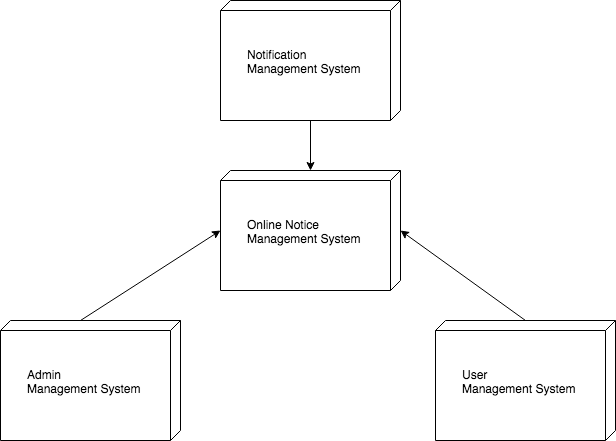
\includegraphics[height=3in]{figures/context_level.png}
    		\caption{Context Level Diagram}
    	\end{figure}
    	
    	\subsubsection{ER Diagram}
    	\begin{figure}[H]
    		\centering
    		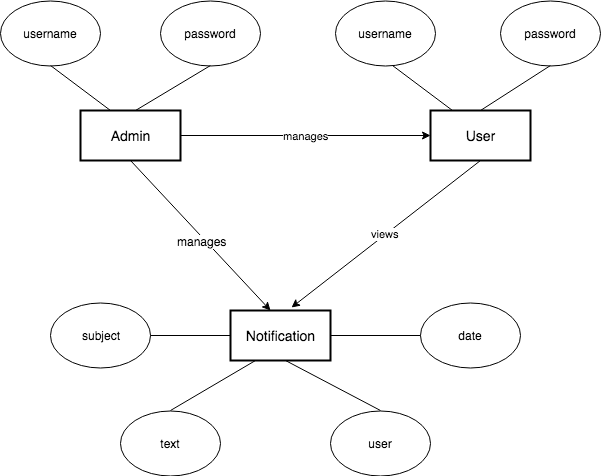
\includegraphics[height=3.5in]{figures/erd.png}
    		\caption{ER Diagram}
    	\end{figure}
	
\newpage
\section{OUTPUT SNAPSHOTS}
    
    \begin{figure}[H]
    	\centering
    	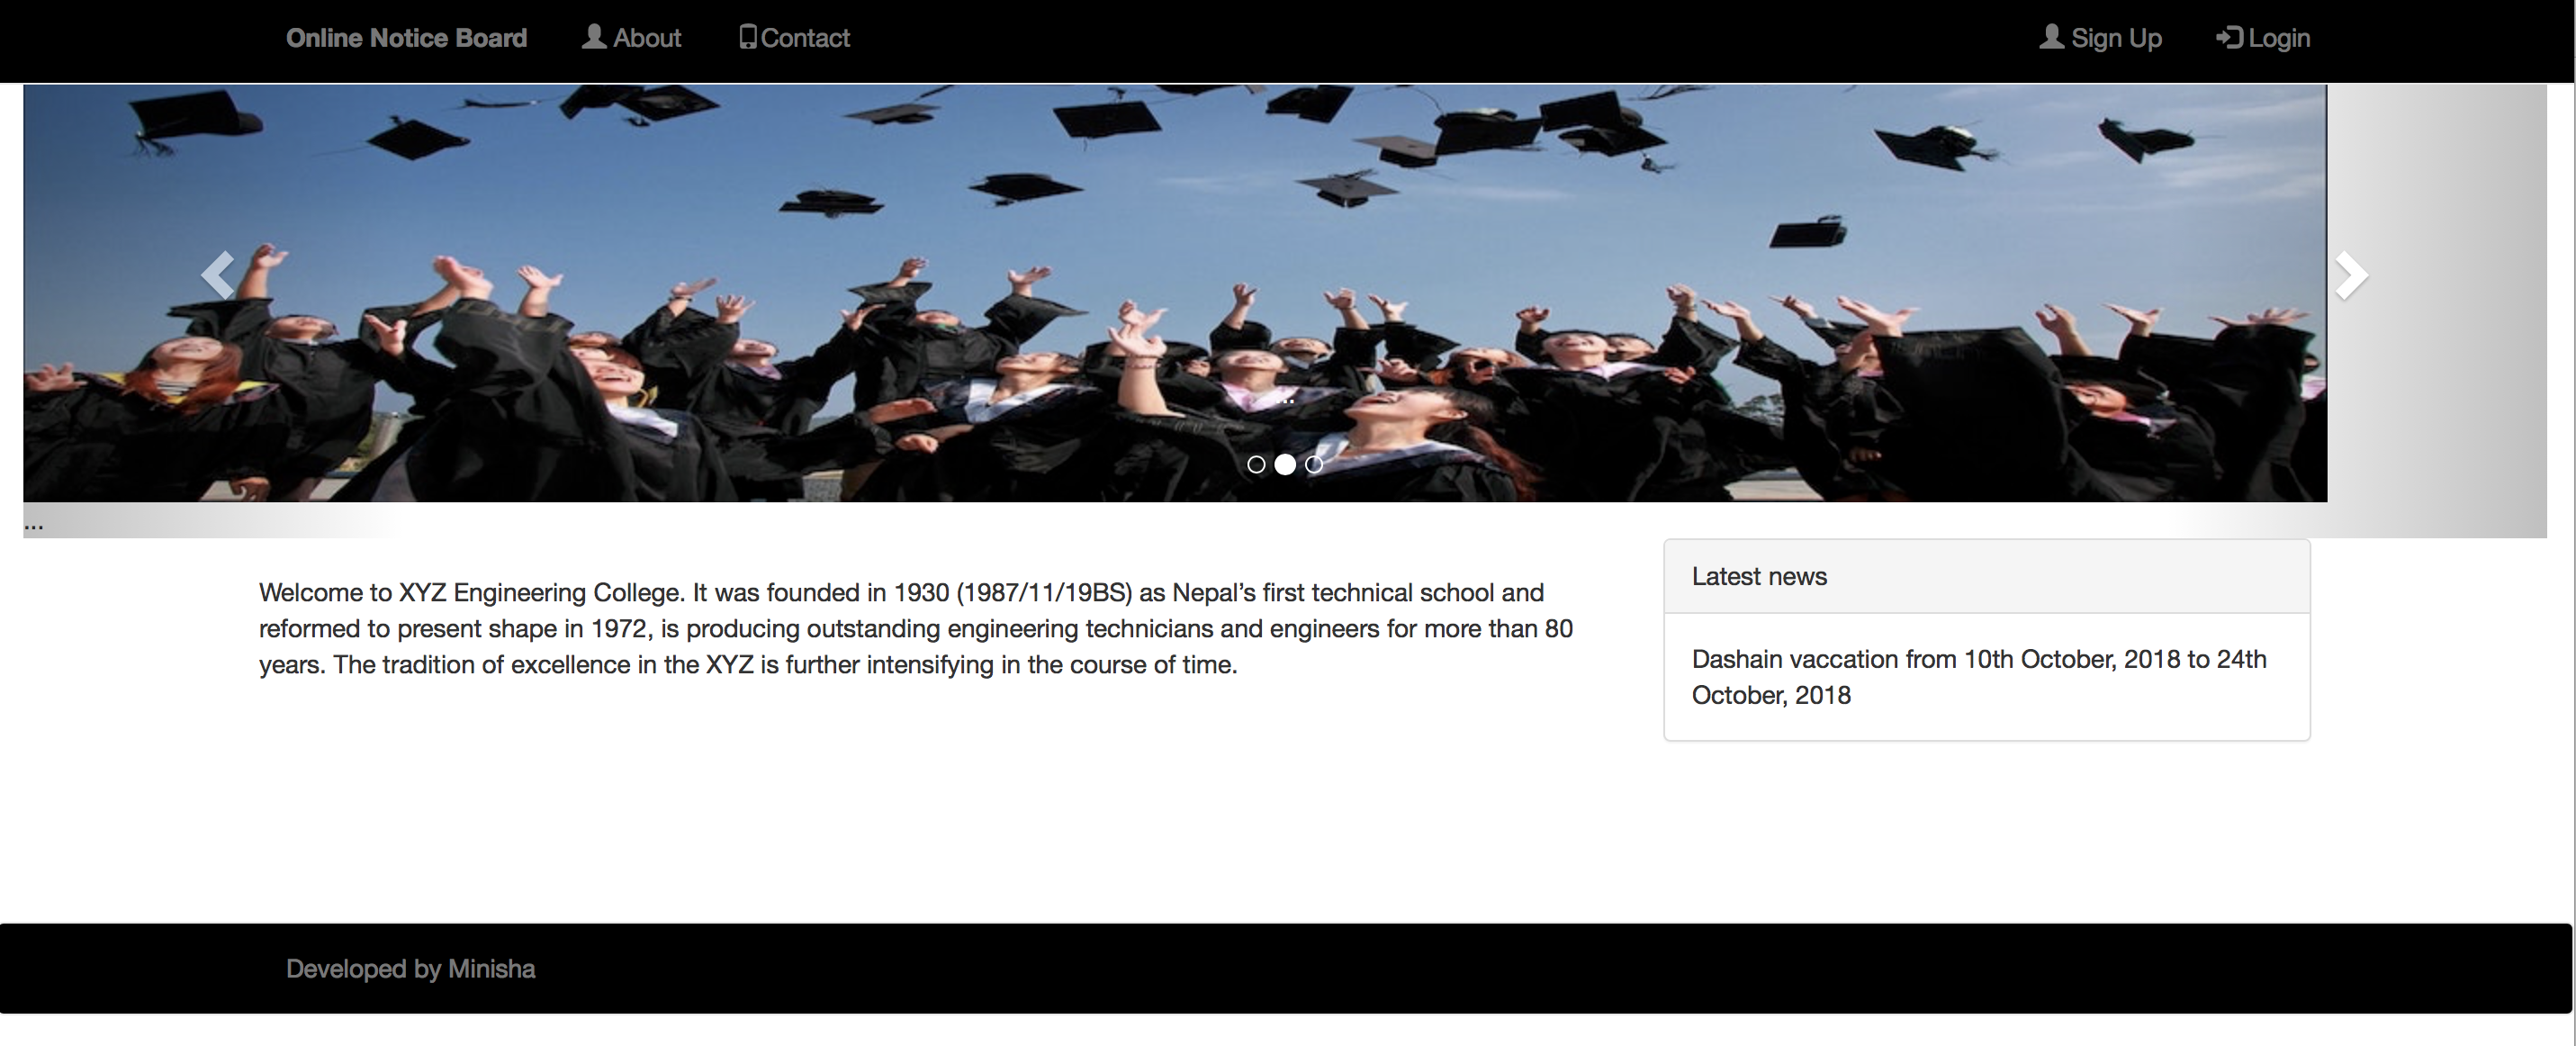
\includegraphics[width=\textwidth,height=2in]{figures/homepage.png}
    	\caption{Home Screen}
    \end{figure}
    
    \begin{figure}[H]
    	\centering
    	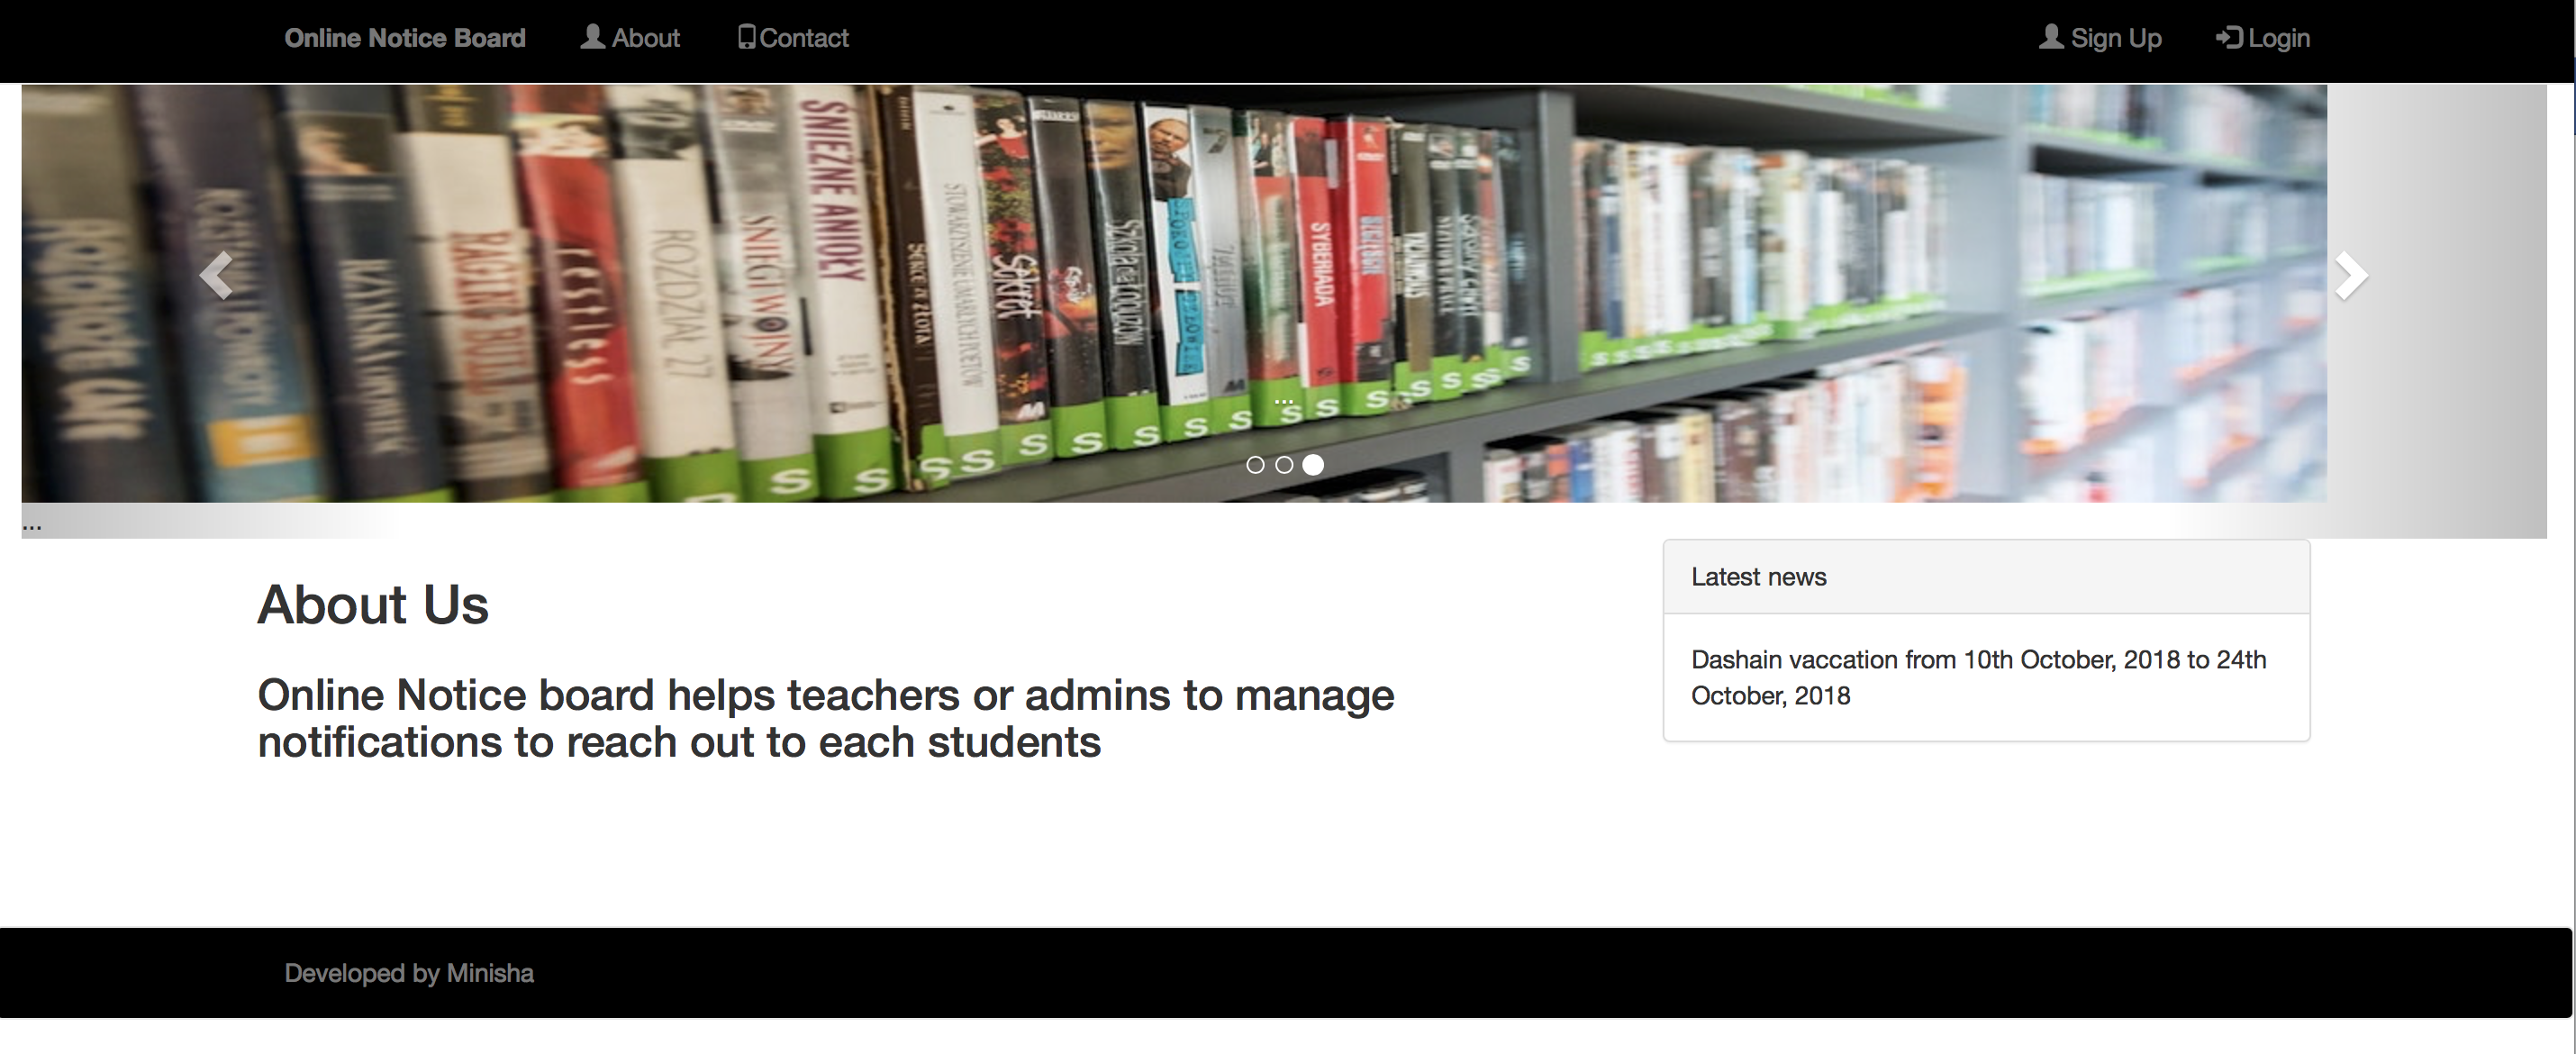
\includegraphics[width=\textwidth,height=2in]{figures/about.png}
    	\caption{About Screen}
    \end{figure}
    
    \begin{figure}[H]
    	\centering
    	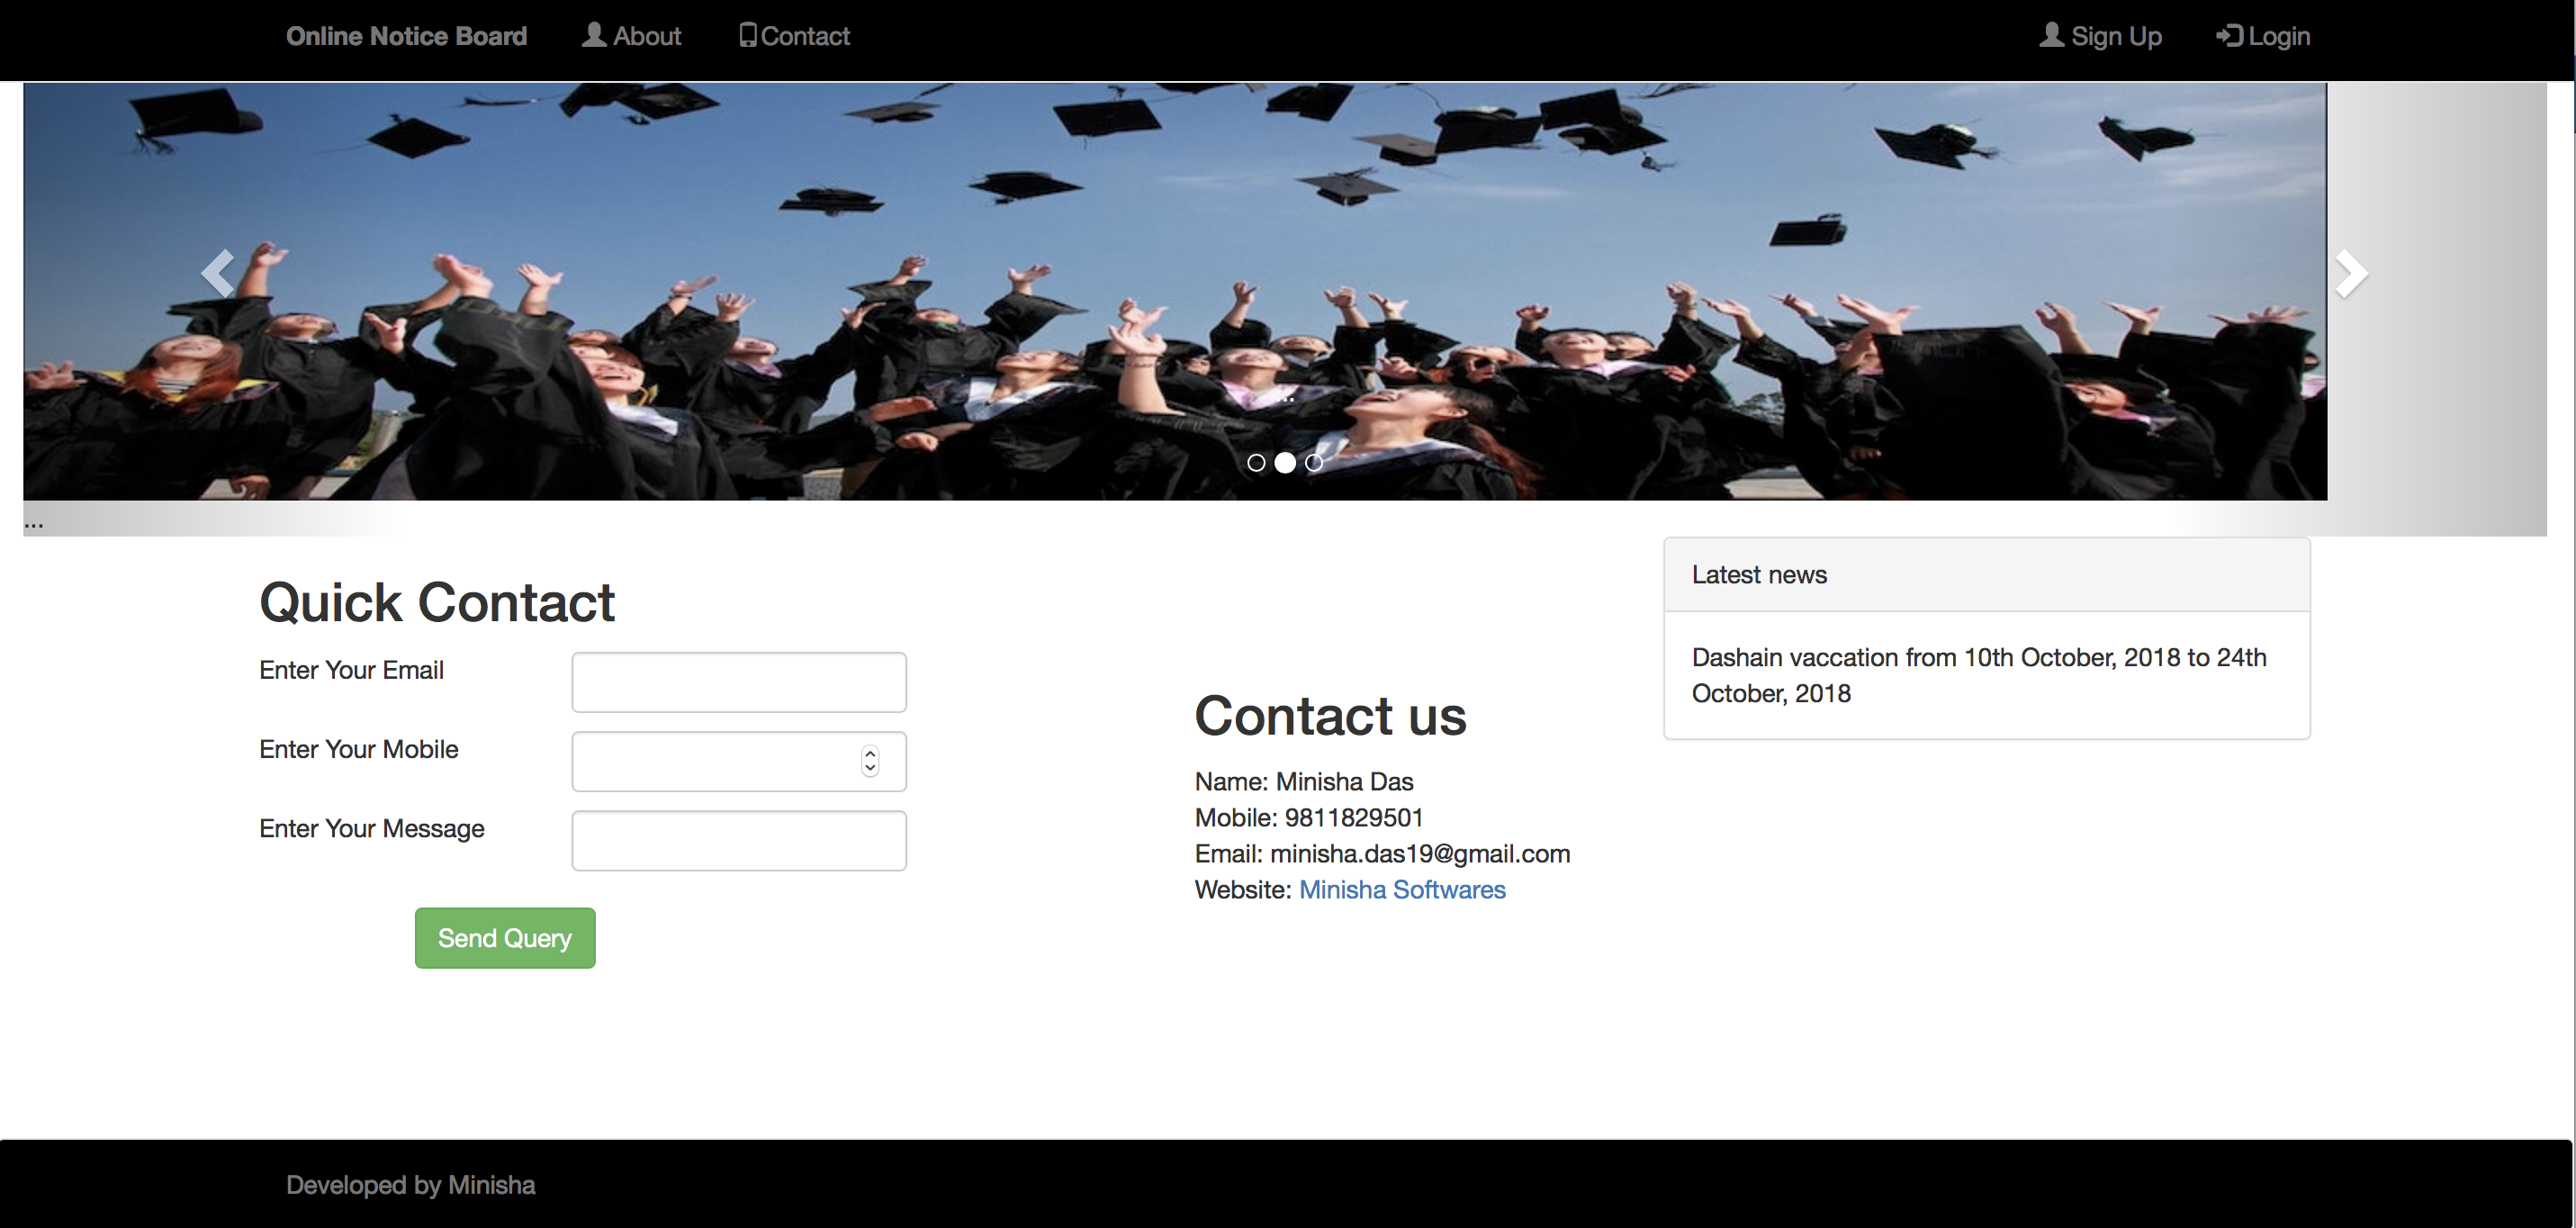
\includegraphics[width=\textwidth,height=2in]{figures/contact.png}
    	\caption{Contact Screen}
    \end{figure}
    
    \begin{figure}[H]
    	\centering
    	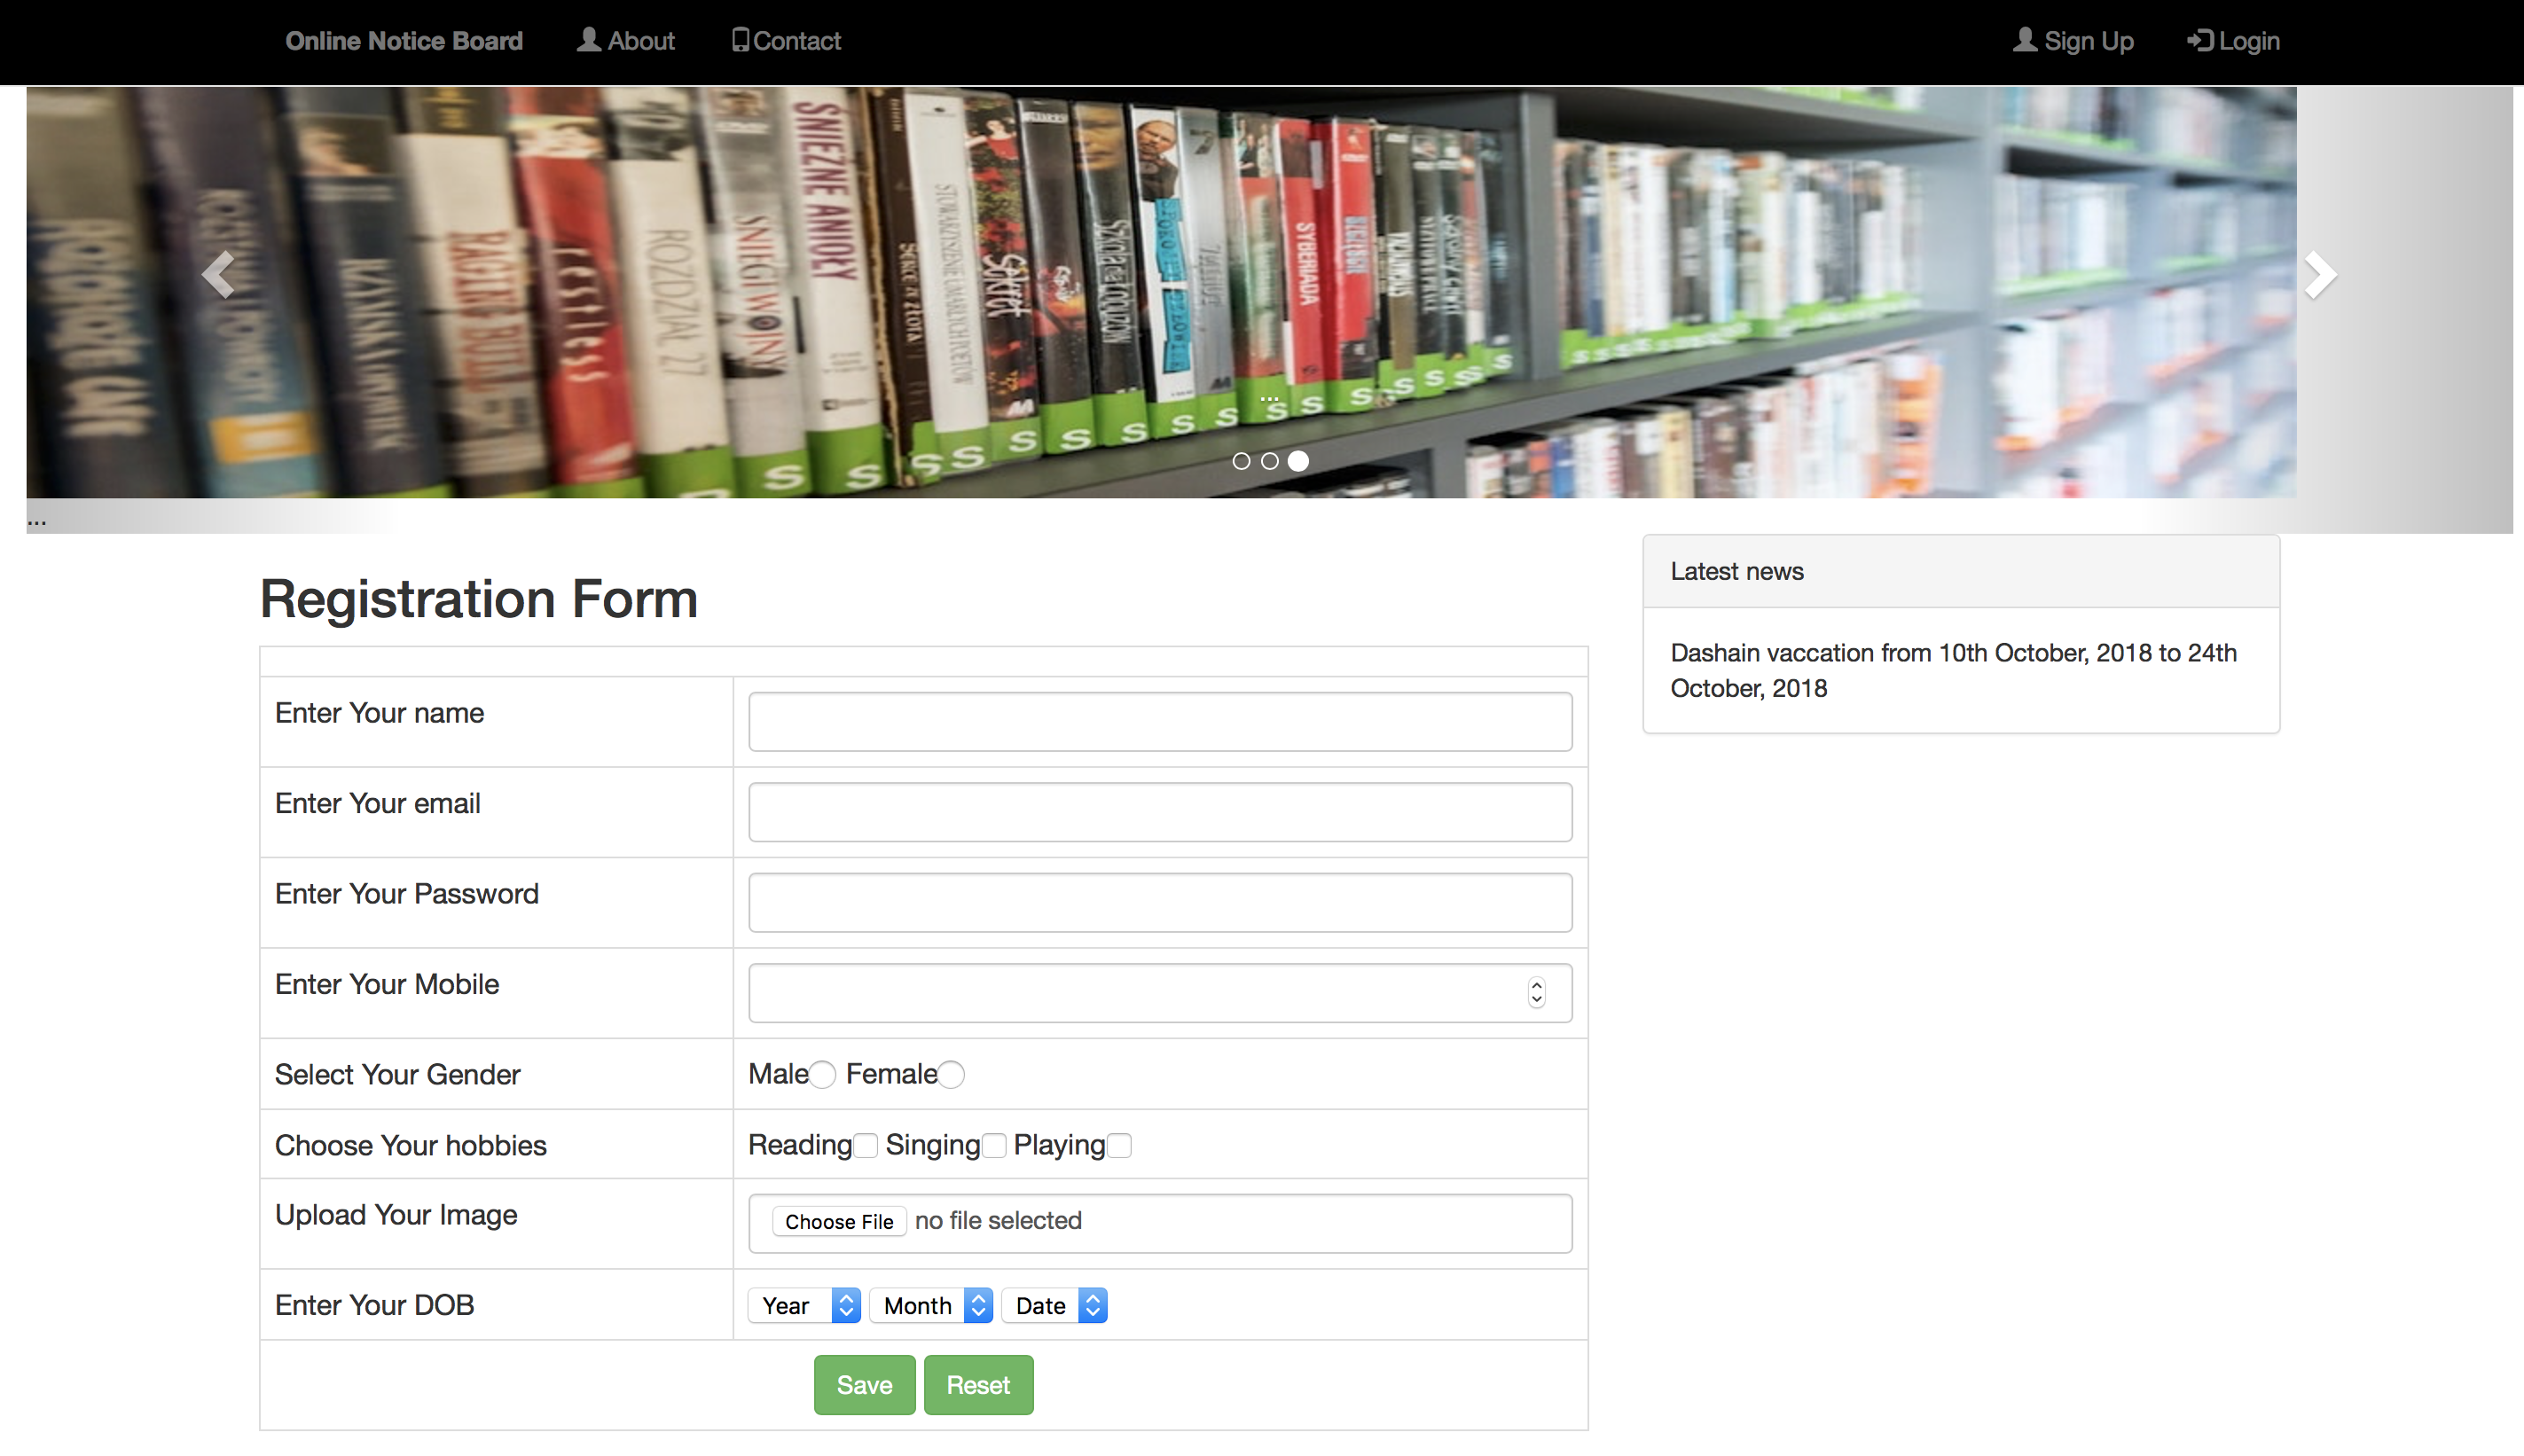
\includegraphics[width=\textwidth,height=2in]{figures/user_registration.png}
    	\caption{User Sign Up Screen}
    \end{figure}
    
    \begin{figure}[H]
    	\centering
    	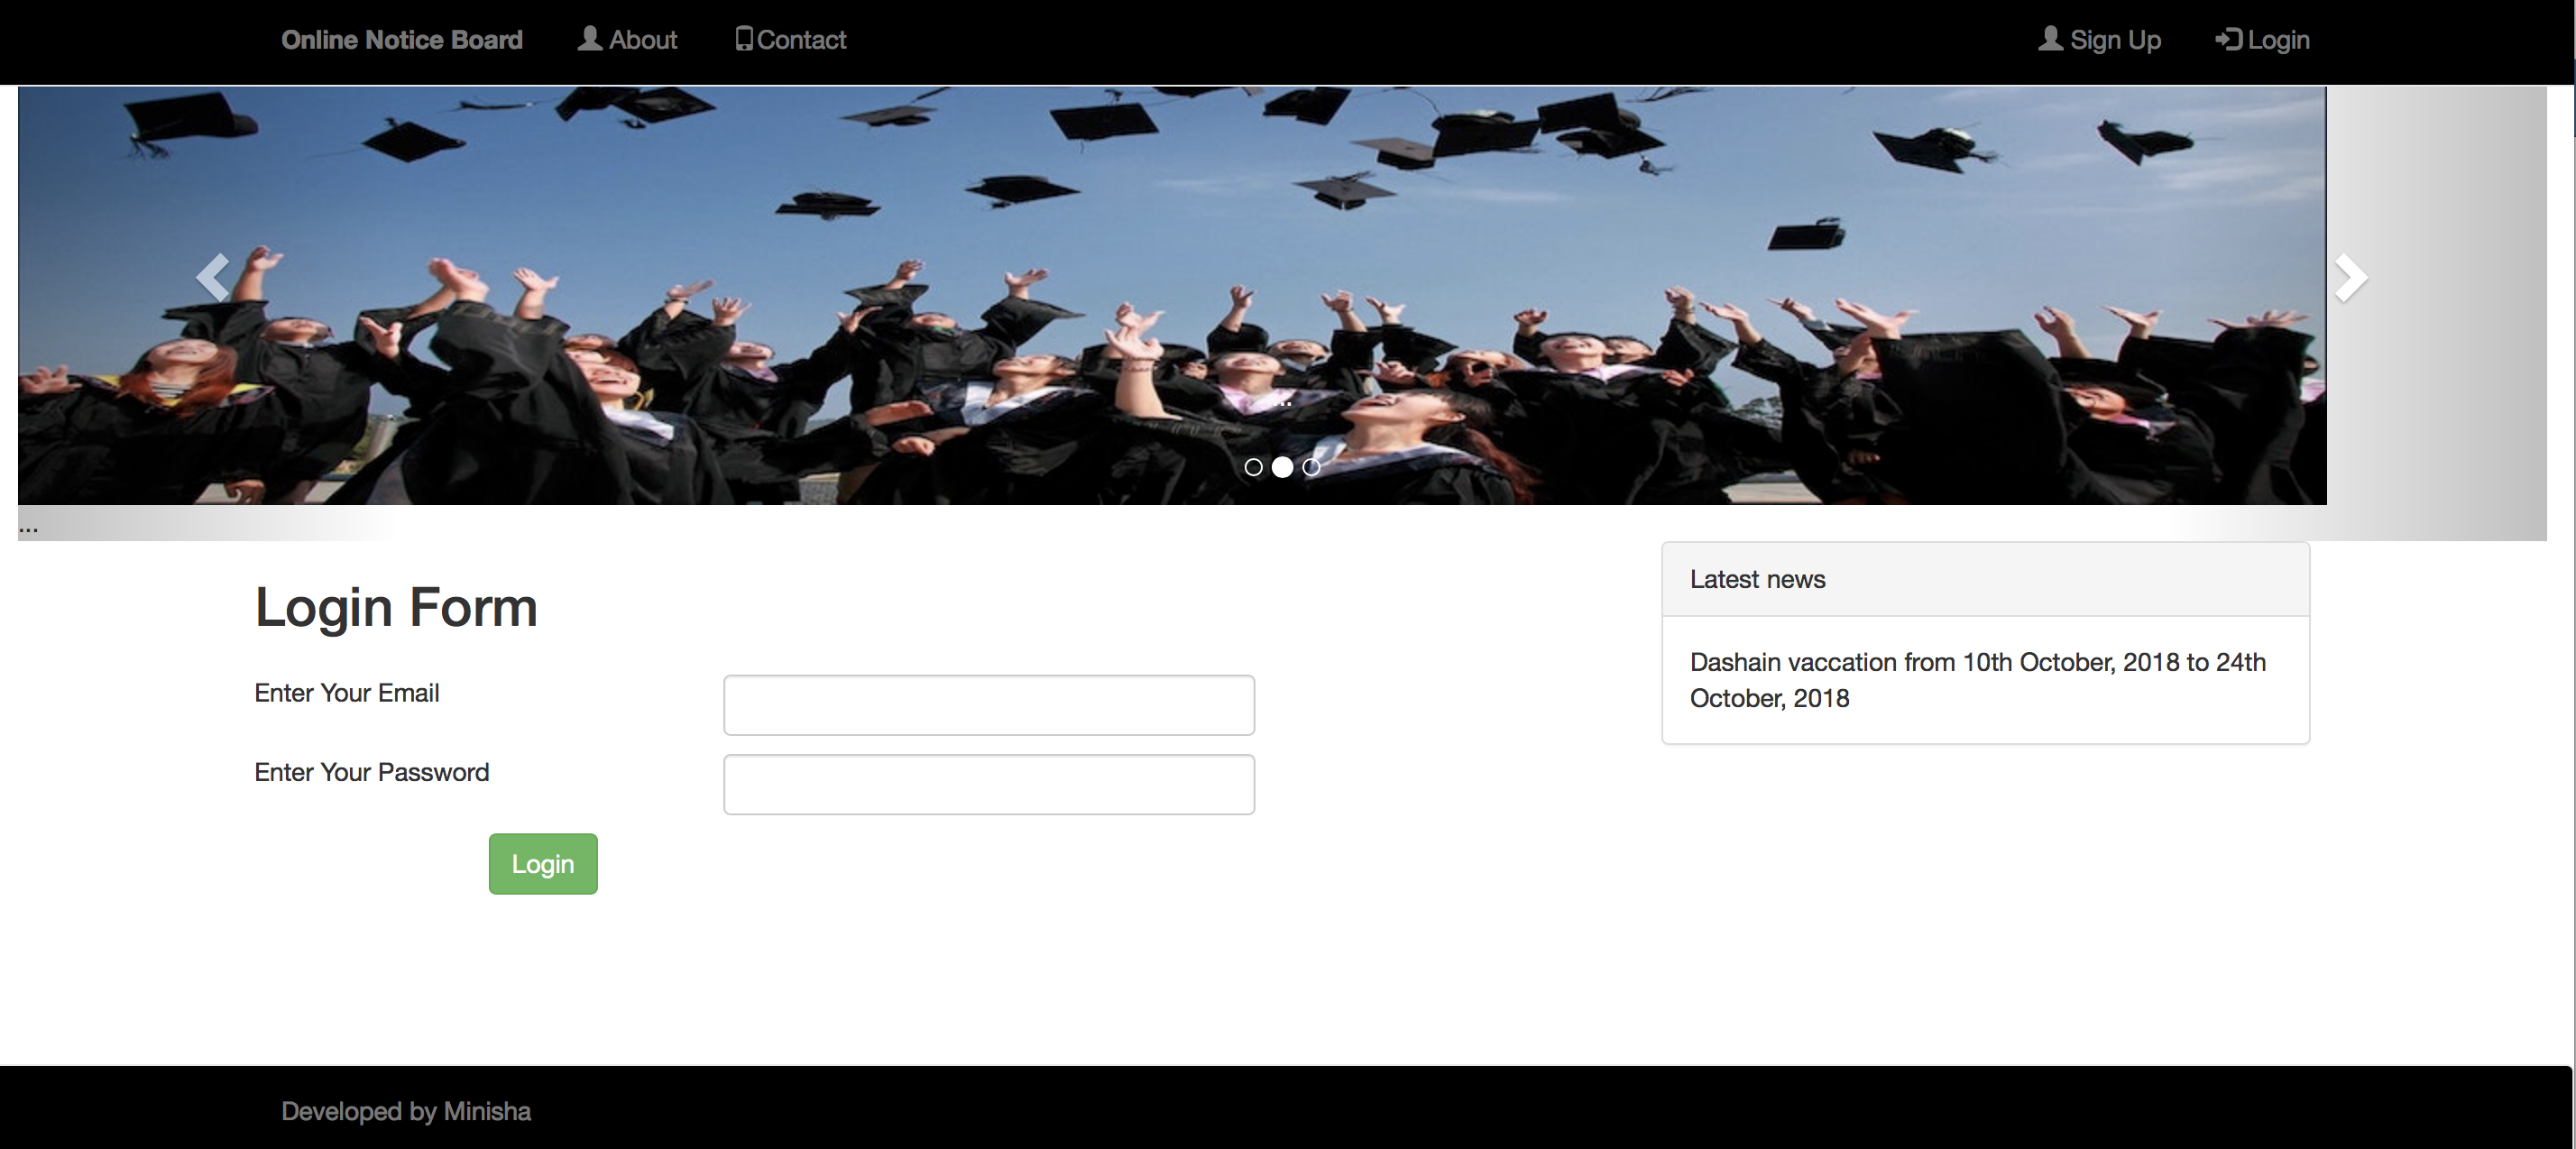
\includegraphics[width=\textwidth,height=2in]{figures/user_login.png}
    	\caption{User Login Screen}
    \end{figure}
    
    \begin{figure}[H]
    	\centering
    	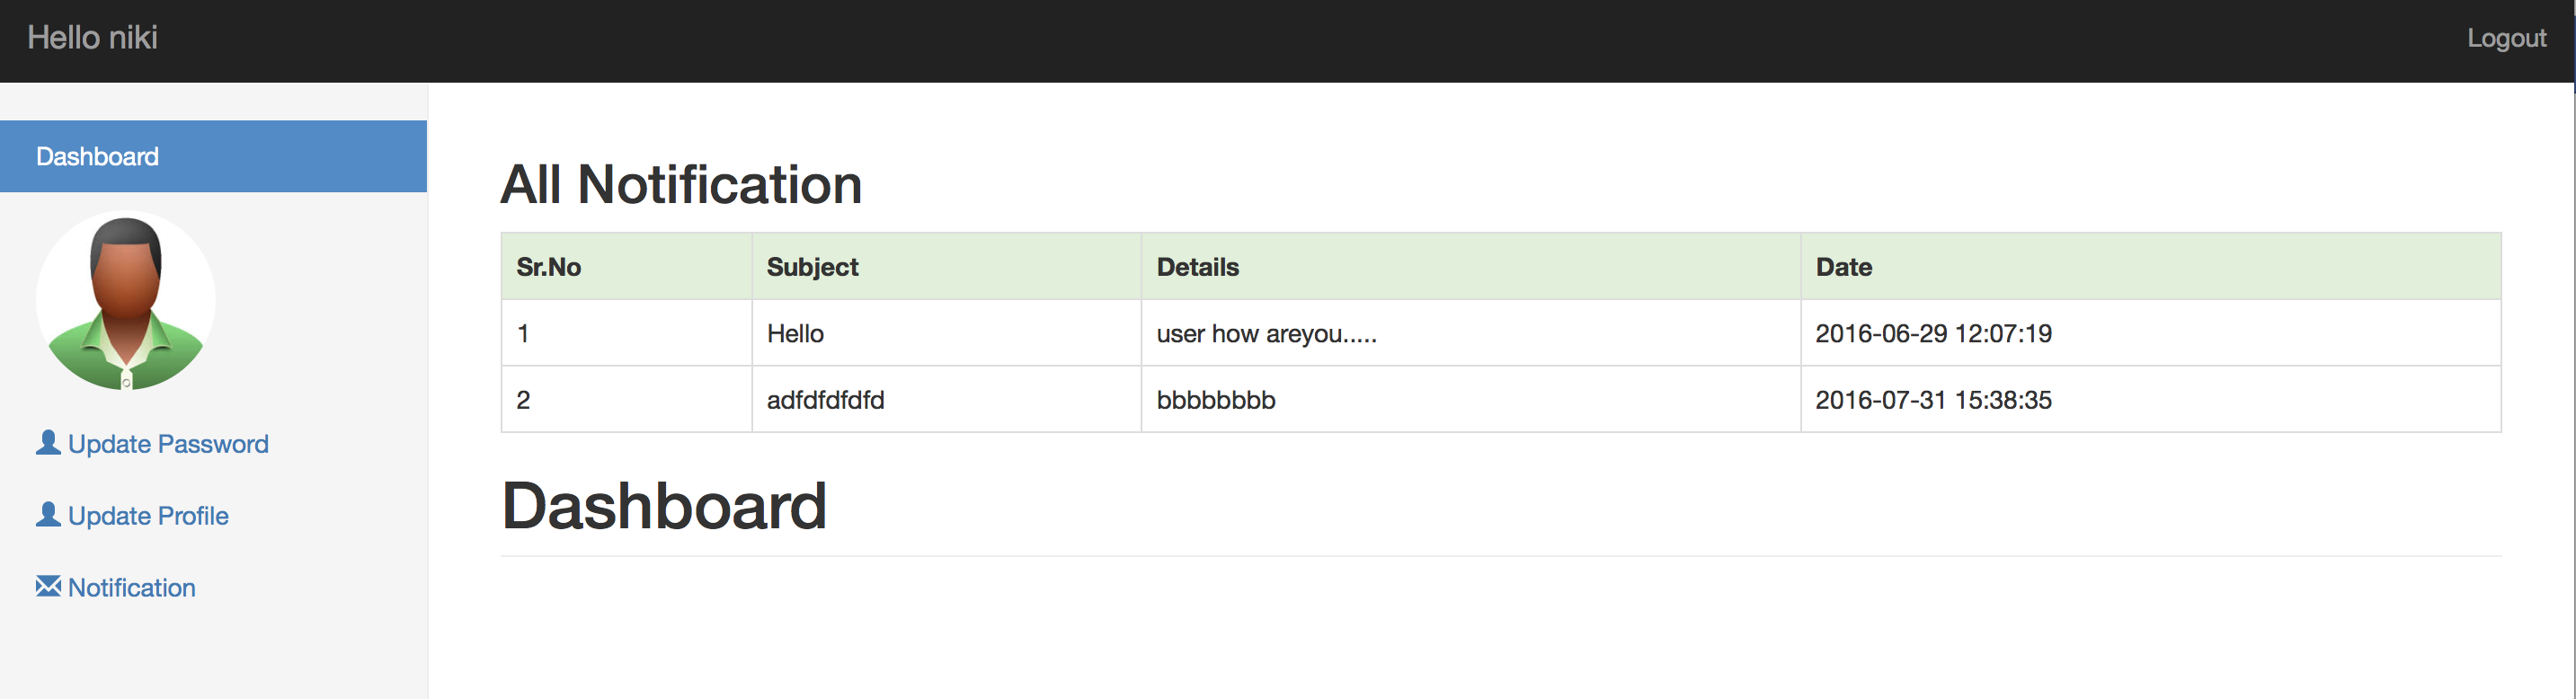
\includegraphics[width=\textwidth,height=2in]{figures/user_dashboard.png}
    	\caption{User Dashboard Screen}
    \end{figure}
    
    \begin{figure}[H]
    	\centering
    	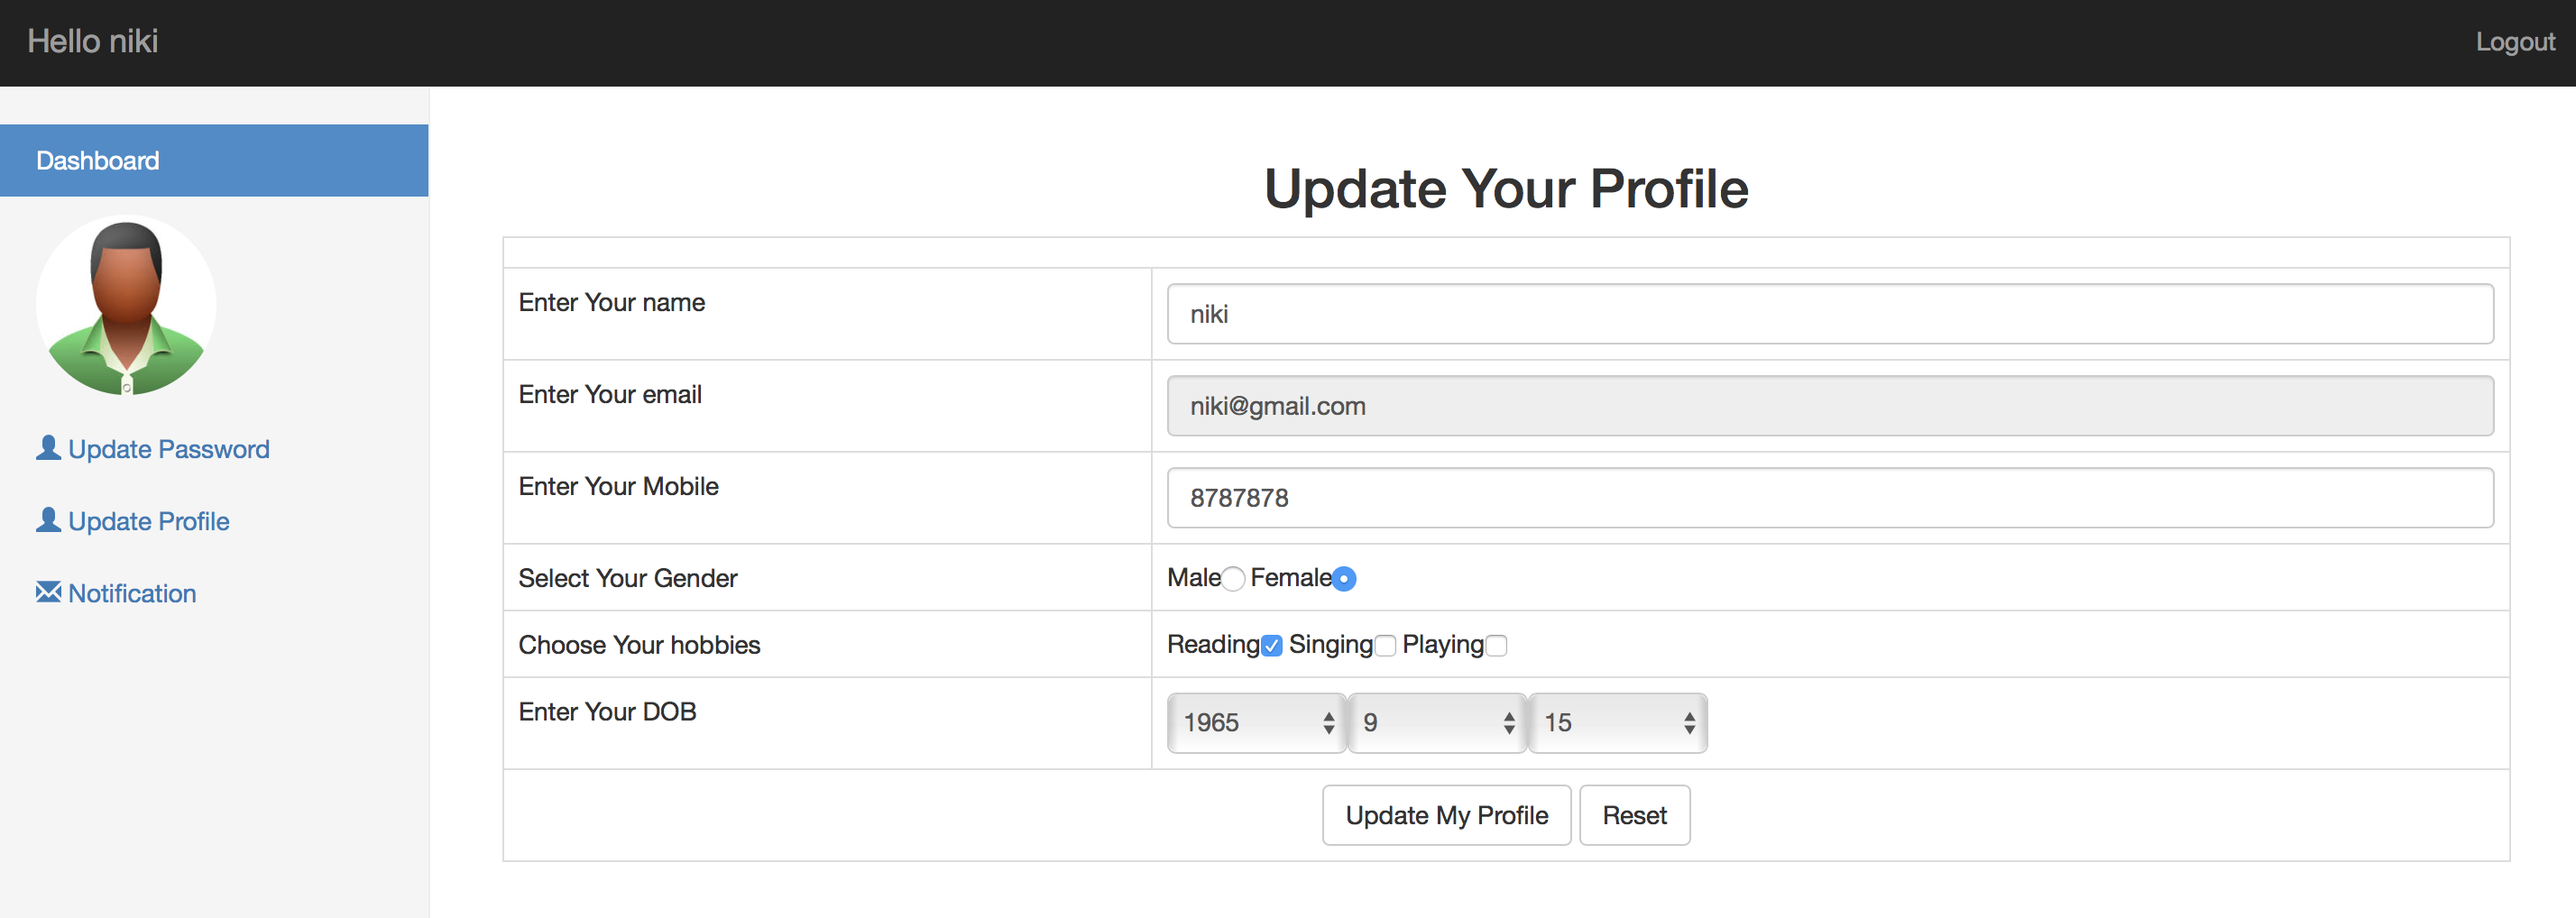
\includegraphics[width=\textwidth,height=2in]{figures/user_update_profile.png}
    	\caption{User Manage Profile Screen}
    \end{figure}
    
    \begin{figure}[H]
    	\centering
    	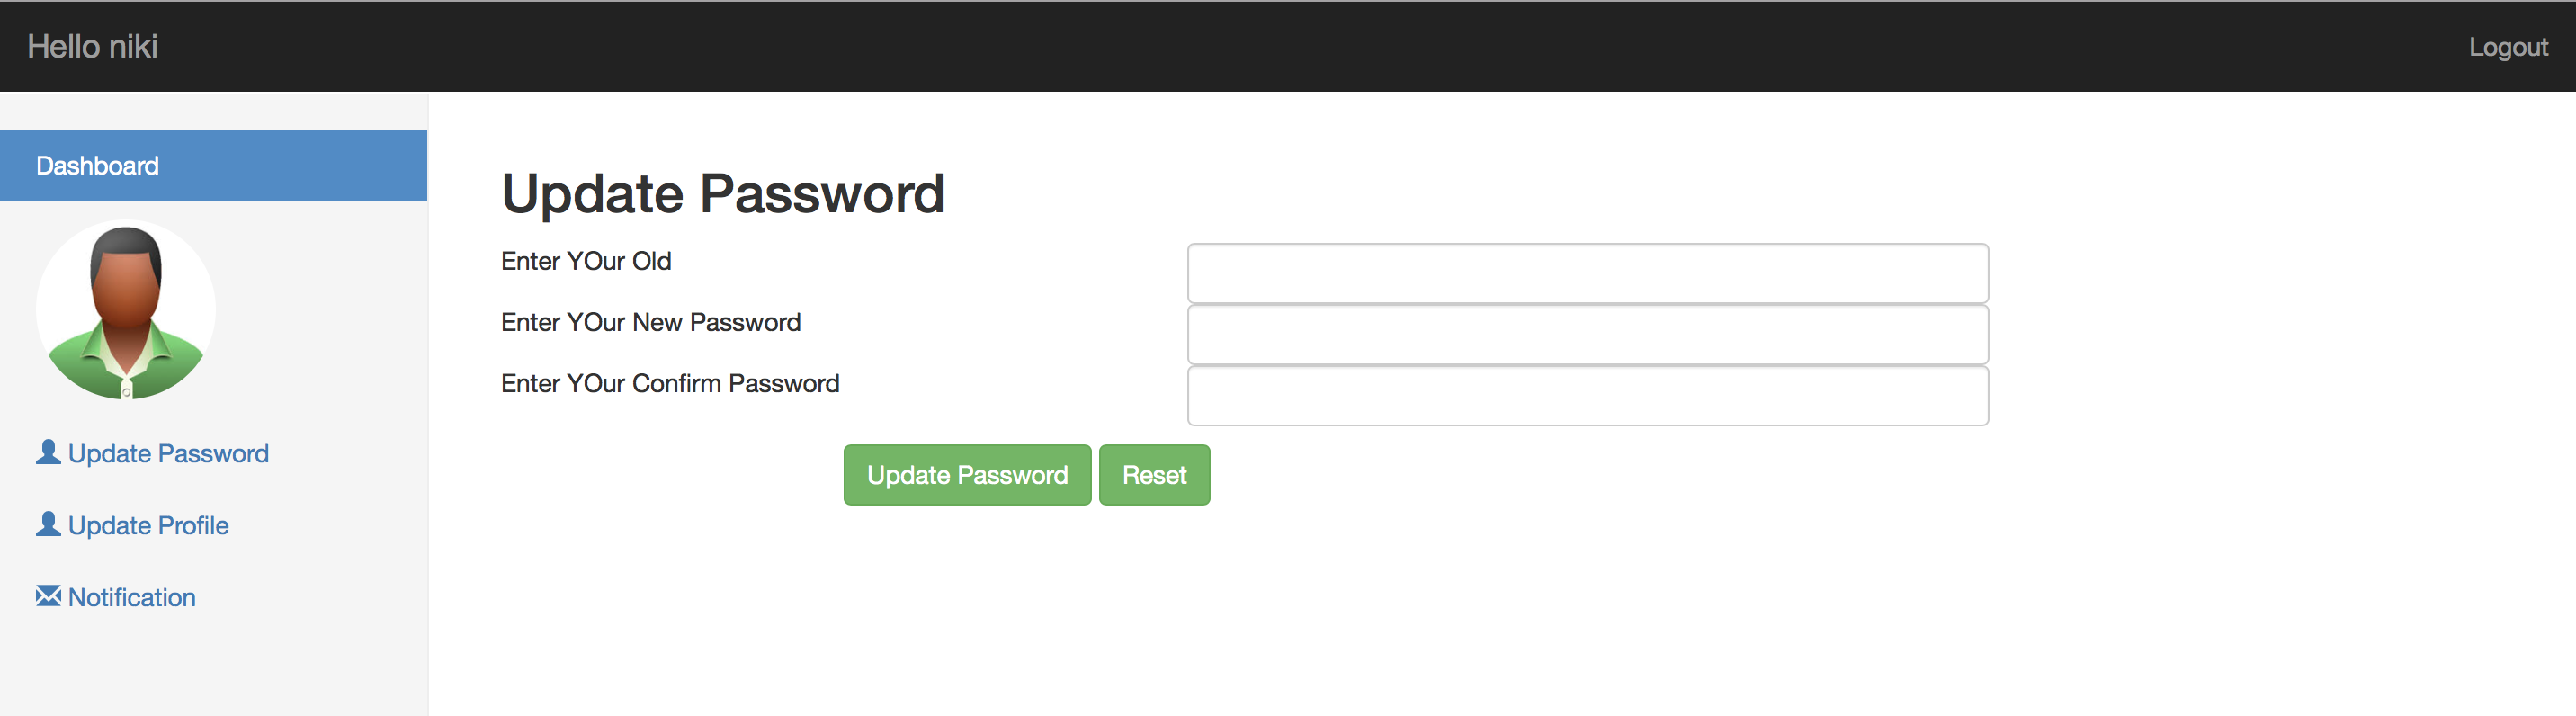
\includegraphics[width=\textwidth,height=2in]{figures/user_update_password.png}
    	\caption{User Manage Password Screen}
    \end{figure}
    
    \begin{figure}[H]
    	\centering
    	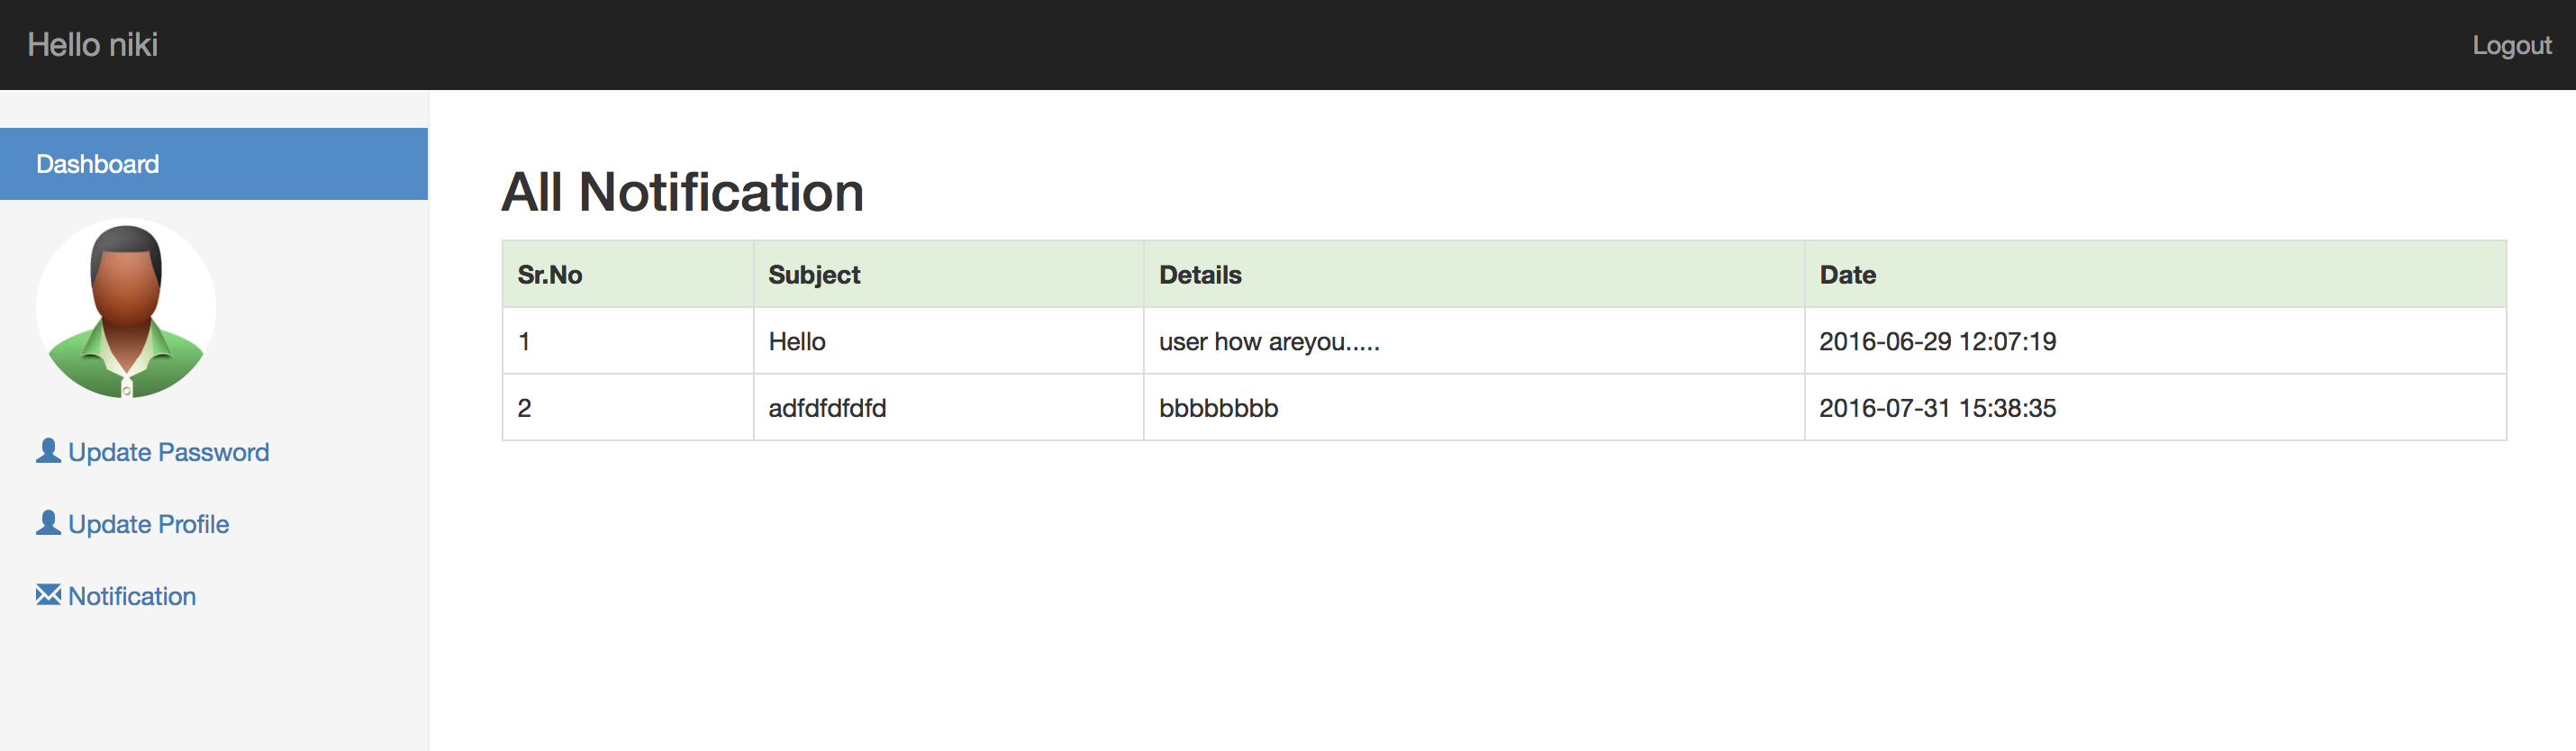
\includegraphics[width=\textwidth,height=2in]{figures/user_view_notification.png}
    	\caption{User View Notifications Screen}
    \end{figure}
    
     \begin{figure}[H]
    	\centering
    	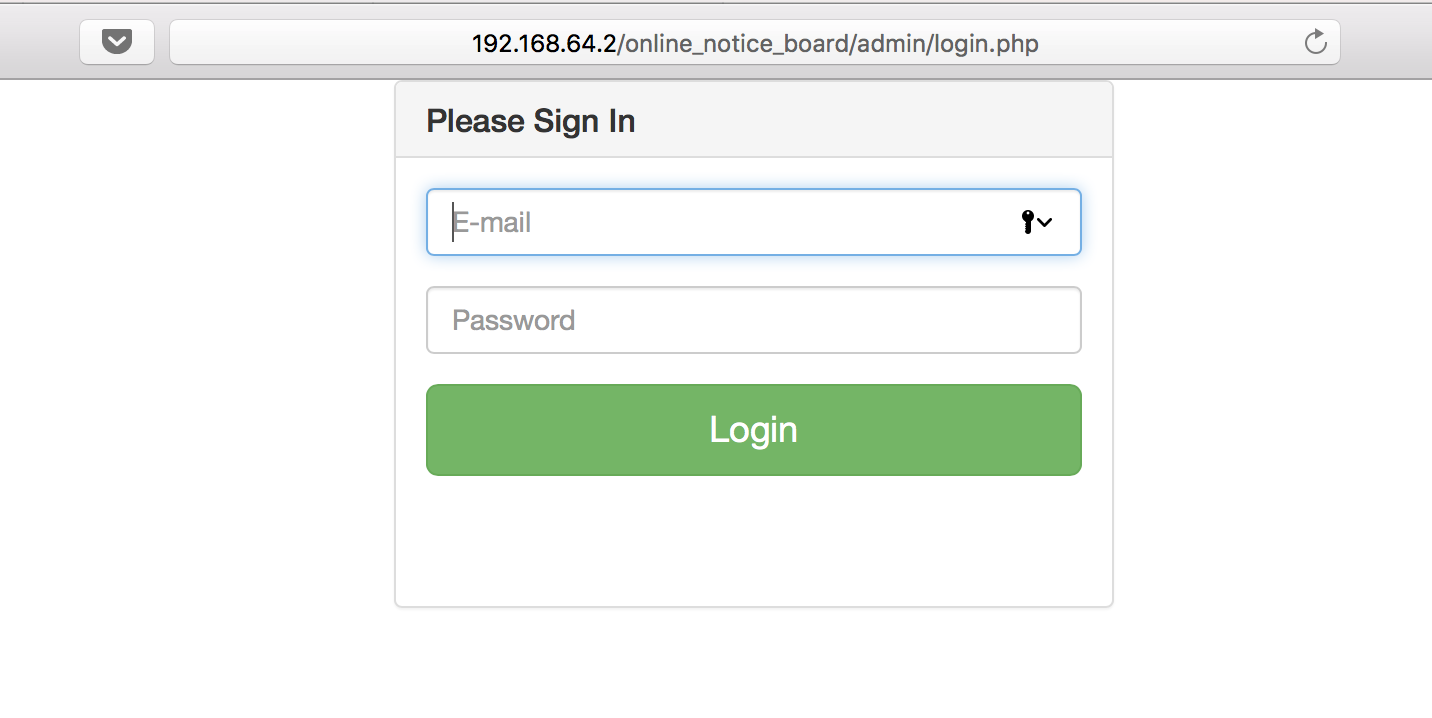
\includegraphics[width=\textwidth,height=2in]{figures/admin_login.png}
    	\caption{Admin Authentication Screen}
    \end{figure}
    
    \begin{figure}[H]
    	\centering
    	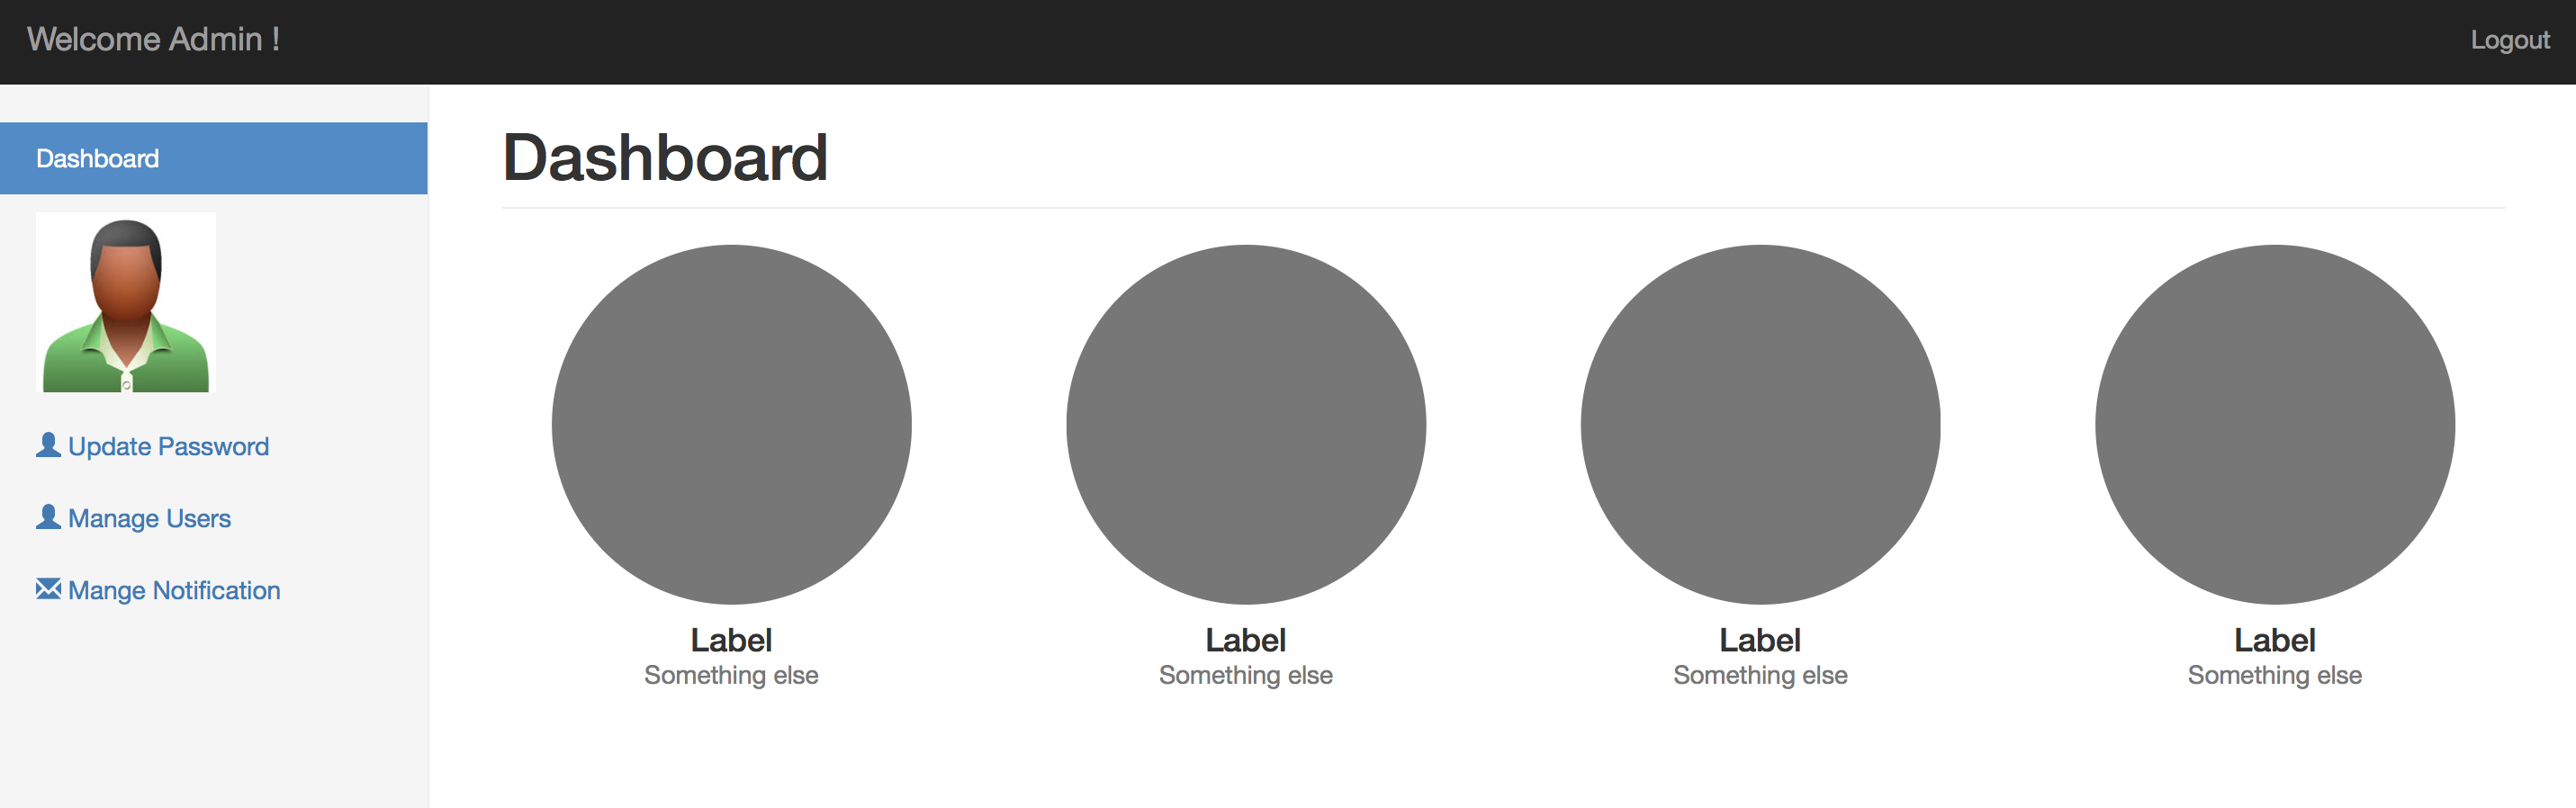
\includegraphics[width=\textwidth,height=2in]{figures/admin_dashboard.png}
    	\caption{Admin Dashboard Screen}
    \end{figure}
    
    \begin{figure}[H]
    	\centering
    	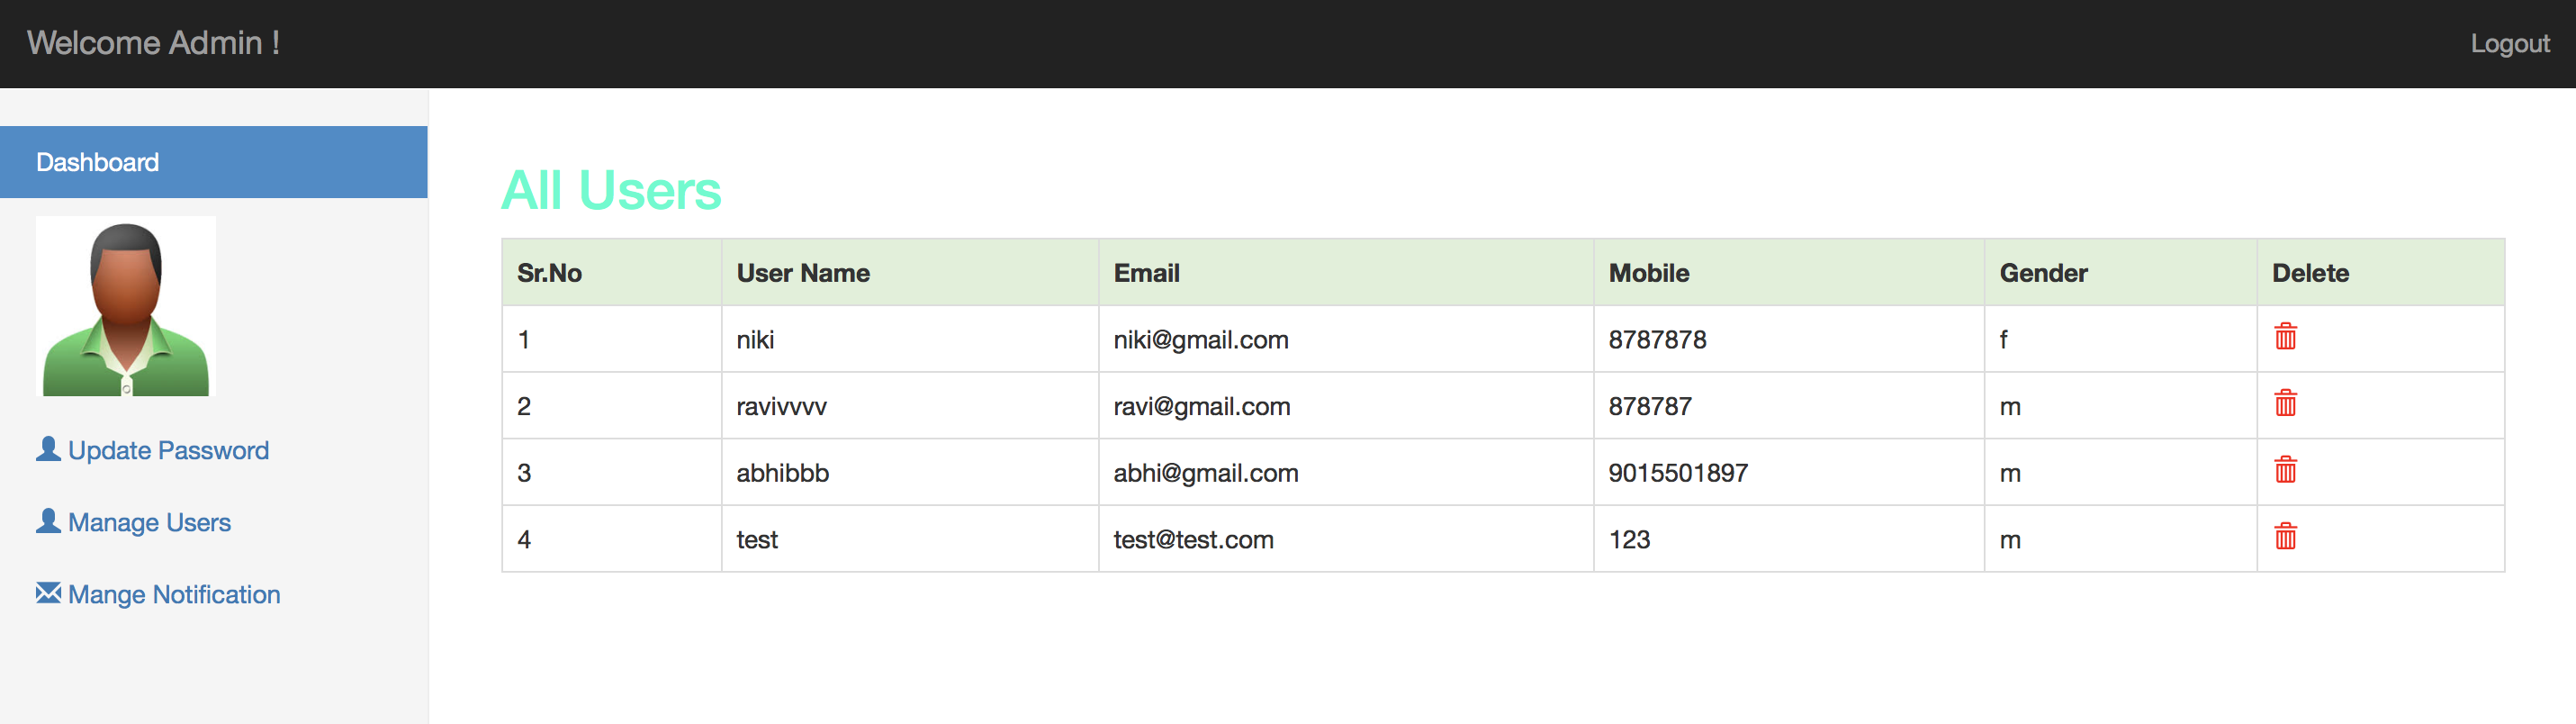
\includegraphics[width=\textwidth,height=2in]{figures/admin_manage_users.png}
    	\caption{Admin Manage Users Screen}
    \end{figure}
    
    \begin{figure}[H]
    	\centering
    	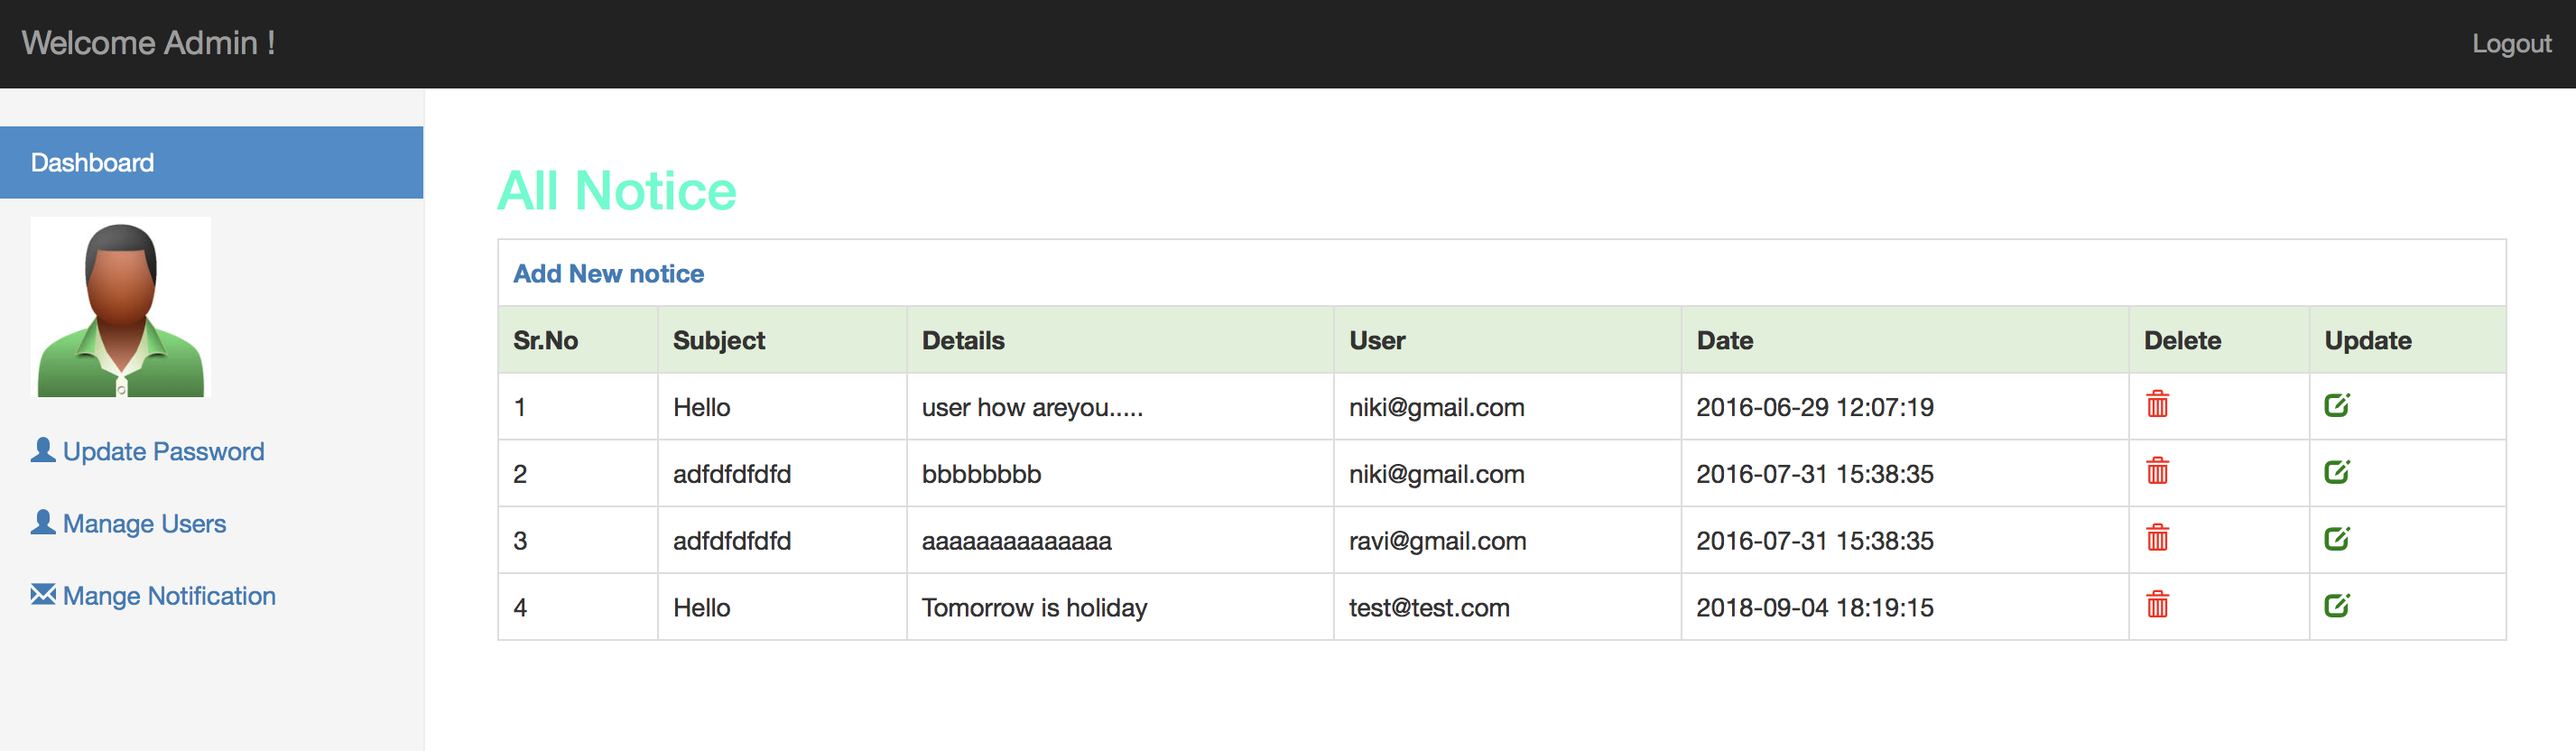
\includegraphics[width=\textwidth,height=2in]{figures/admin_view_all_notice.png}
    	\caption{Admin Manage Notification Screen}
    \end{figure}
    
    \begin{figure}[H]
    	\centering
    	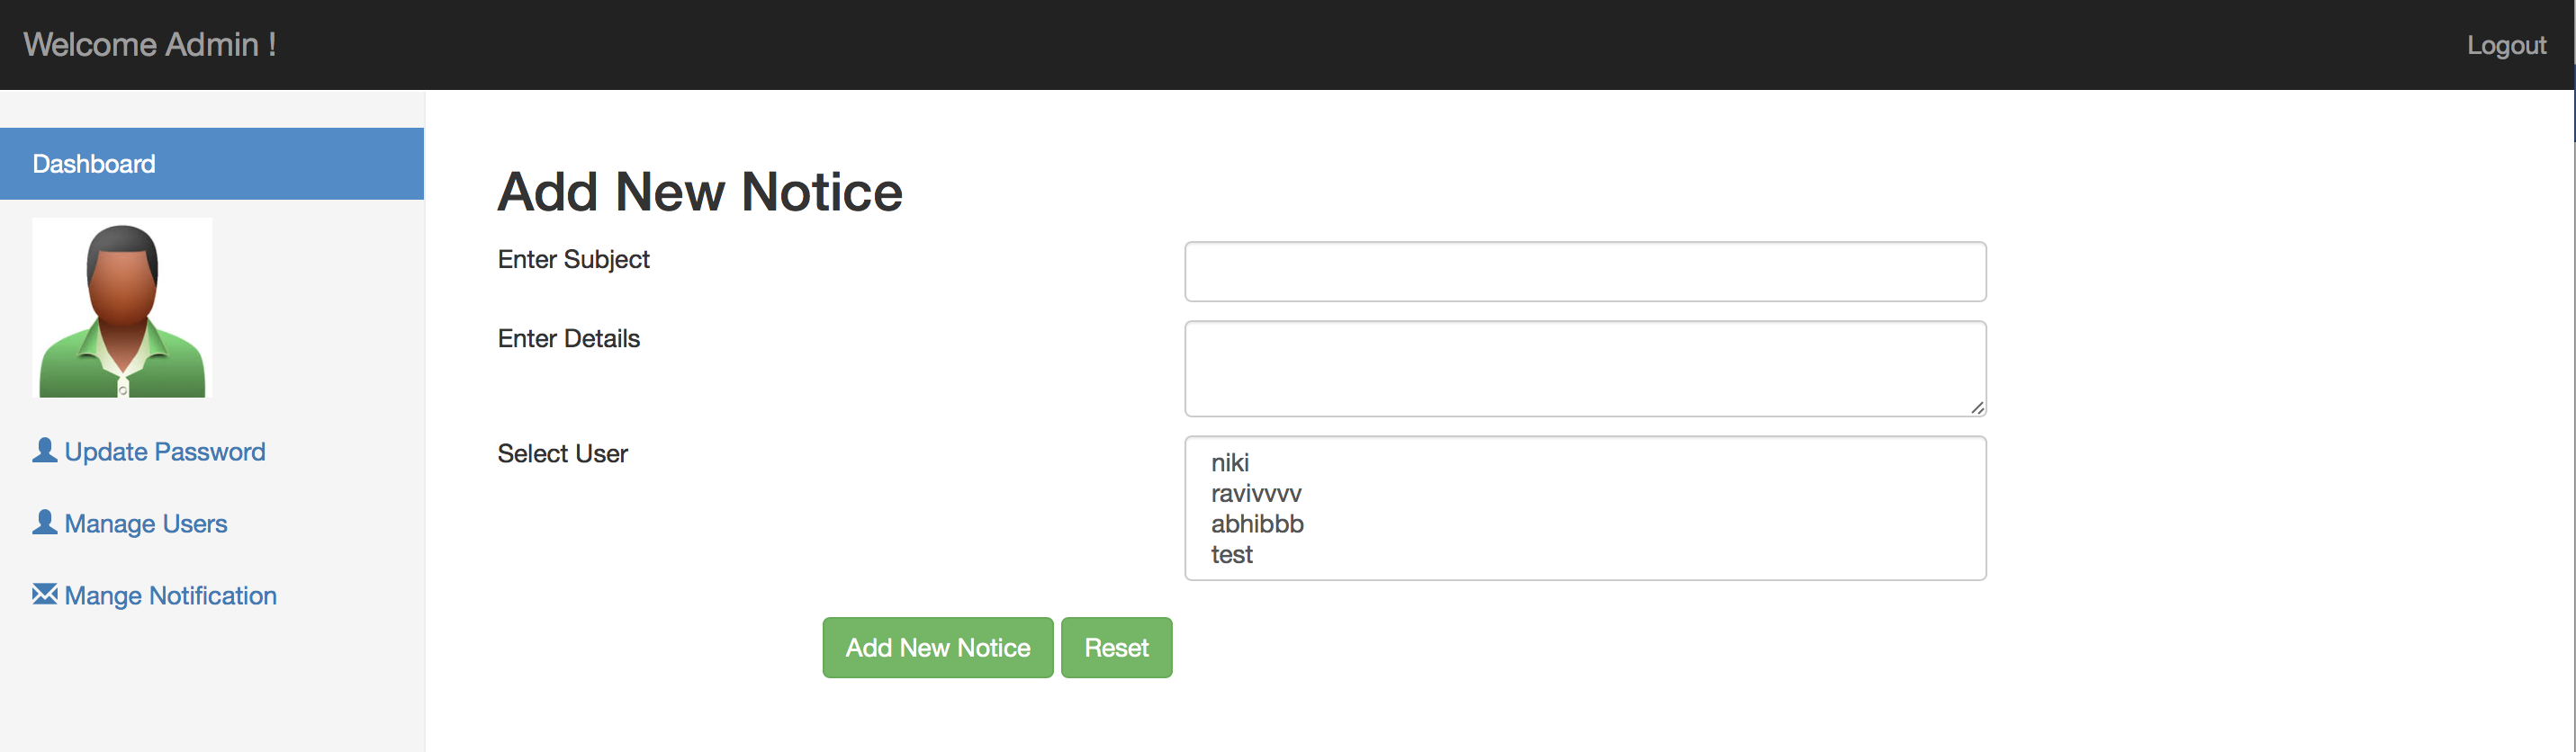
\includegraphics[width=\textwidth,height=2in]{figures/admin_add_notice.png}
    	\caption{Admin Add Notice Screen}
    \end{figure}
    
\newpage
\section{CONCLUSION AND FURTHER ENHANCEMENTS}
The main aim of our project was to reflect whatever we have learned in our Computer Engineering. With this motive, we intended to develop a Online Notice Board system that automates the notice management and incidents process. During our project, we became  familiar with programming techniques and software development process.\\
Although we have tried our best to simulate the notice board work-flow, there are still much rooms for improvements of our project. In the future, we may be able to implement following functionality:
\begin{itemize}
    \item Add group users to intend a notice to a group of students.
    \item Better database management
    \item Scaling by implementing better client-server architecture.
\end{itemize}
With whatever we have learned till now, we tried our best to implement it practically. We will try to improve our practice in future projects.

\newpage
\bibliographystyle{plain}
\bibliography{REFERENCES}
\addcontentsline{toc}{section}{\numberline{}REFERENCES}

\end{document}